\chapter{Predictive Coding}

\section{Introduction}

In this chapter, we consider the application of the free energy principle to perception. Here, we focus entirely on visual perception and the process theory of predictive coding \citep{friston2003learning,friston2005theory,bastos2012canonical,buckley2017free,spratling2017review}. This chapter is organized into four relatively independent sections which each present a separate piece of work, which extends or contributes to the theory or practice of predictive coding. The general theme of our work aims to scale up predictive coding to reach the levels of performance achieved by machine learning, as well as to understand the potential biological plausibility of the theory. Both of these are important for understanding the potential predictive coding has as a general theory of cortical function since, if it is actually implemented in the brain, it must meet both bars of extremely high scalability (since the brain effortlessly handles perception and inference with extremely detailed and complex inputs, as well as constructing extremely powerful and general representations), as well as the biological plausibility necessary to allow the dynamics prescribed by predictive coding to be implemented by neural circuitry.

We begin with a mathematical introduction to predictive coding and its dynamics. This is followed with the presentation of our work where we experiment with implementing larger scale predictive coding networks than previously in the literature, and validate their performance and capabilities on benchmark machine learning datasets -- thus demonstrating that predictive coding as a theory can be scaled up to the standards of modern deep learning. We also experiment with dynamical predictive coding networks using generalized coordinates (as introduced \citep{friston2008DEM}) as well as combining both hierarchical and dynamical predictive coding networks, although these implementations are only tested on relatively small toy tasks and scaling these up to larger and much more challenging dynamical tasks, such as video prediction, remains an important avenue for future work.

In the second section, we focus on understanding how predictive coding can be written as a filtering algorithm -- and thus can be applied productively to fundamentally dynamical instead of static stimuli. We demonstrate precisely how predictive coding is related to Kalman filtering -- a ubiquitous and extremely successful Bayesian filtering algorithm \citep{kalman1960contributions,kalman1961new} -- and also show how predictive coding can extend this algorithm to allow for the online learning of the parameters of the generative model (as well as inference of the states) -- a capability which is not usually achieved with Kalman filtering alone. We validate the performance of this algorithm on simple filtering tasks.

%Thirdly, we (-/cite hybrid inference)

Fourthly, we investigate the biological plausibility of predictive coding, show how the standard model possesses three key implausibilities -- weight transport, nonlinear derivatives, and one-to-one error unit connectivity, and show how each can be overcome with biologically plausible additions to the algorithm without causing much of a degradation in the classification performance of the algorithm.

%In this chapter, we shift gears somewhat from the previous chapters which focused on deep active inference, and the application of methods inspired by the Free Energy Principle to control problems -- and specifically the mathematical origin of exploration. In the next two chapters, instead, we focus applications of the Free Energy Principle to questions in neuroscience. In this chapter, we deeply explore theories of predictive coding \citep{mumford1992computational,rao1999predictive,spratling2017review,friston2003learning,friston2008hierarchical}. Specifically, we focus firstly on our initial work in implementing large-scale predictive coding networks and testing them on machine learning tasks. We then, in joint work with Alexander Tschantz, formulate predictive coding networks in terms of iterative and amortized inference, and experiment with adding a feedforward `amortised' sweep to a standard predictive coding network and show that this `hybrid' network has substantially improved computational properties compared to purely iterative predictive coding. Next, we investigate the relationship between predictive coding as applied to Bayesian filtering problems and the classical Kalman filter \citep{kalman1960new}, where we show that predictive coding can be understood as optimizing the same objective as the Kalman filter but performs a gradient descent on this objective while the Kalman filter solves the optimization problem analytically. Finally, we improve the biological plausibility of the predictive coding algorithm by proposing several changes to the algorithm which do not unduly reduce performance while correcting several biologically implausible aspects.

%In the next chapter we continue our discussion on the  applications of the Free-Energy principle to neuroscience by investigating how predictive coding can aid us in understanding the open and challenging problem of biologically plausible \emph{credit assignment} in the brain. We first demonstrate \citep{millidge2020predictive} how predictive coding, under certain conditions, can approximate the widely utilized backpropagation of error algorithm \citep{linnainmaa1970representation,rumelhart1986learning} central to all contemporary machine learning \citep{goodfellow2016deep}, and secondly use insights and intuitions from predictive coding to develop novel and more elegant algorithm to tackle the credit assignment problem in the brain \citep{millidge2020activation,millidge2020investigating}.

\section{Predictive Coding}

Predictive coding is an influential theory in computational and cognitive neuroscience, which proposes a potential unifying theory of cortical function \citep{friston2003learning,friston2005theory,rao1999predictive,friston2010free,clark2013whatever,seth2014cybernetic} -- namely that the core function of the brain is simply to minimize prediction error, where the prediction errors denote mismatches between predicted input and the input actually received. This minimization can be achieved in multiple ways: through immediate inference about the hidden states of the world, which can explain perception \citep{beal2003variational}, through updating a global world-model to make better predictions, which could explain learning \citep{friston2003learning,neal1998view}, and finally through action to sample sensory data from the world that conforms to the predictions \citep{friston2009reinforcement}, which potentially provides an account adaptive behaviour and control. Prediction error minimization can also be influenced by modulating the \emph{precision} (or inverse variance) of sensory signals, which may shed light on the neural implementation of attention mechanisms \citep{feldman2010attention,kanai2015cerebral}. Predictive coding boasts an extremely developed and principled mathematical framework, which formulates it as a variational inference algorithm \citep{blei2017variational,ghahramani2000graphical, jordan1998introduction}, alongside many empirically tested computational models with close links to machine learning \citep{beal2003variational,dayan1995helmholtz,hinton1994autoencoders}, which address how predictive coding can be used to solve challenging perceptual inference and learning tasks similar to those faced by the brain. Moreover, predictive coding also has been translated into neurobiologically plausible microcircuit process theories \citep{bastos2012canonical,shipp2016neural,shipp2013reflections} which are increasingly supported by neurobiological evidence \citep{walsh2020evaluating}. Predictive coding as a theory is also supported by a large amount of empirical evidence and offers a single mechanism that accounts for diverse perceptual and neurobiological phenomena such as end-stopping \citep{rao1999predictive}, bistable perception \citep{hohwy2008predictive,weilnhammer2017predictive}, repetition suppression \citep{auksztulewicz2016repetition}, illusory motions \citep{lotter2016deep,watanabe2018illusory}, and attentional modulation of neural activity \citep{feldman2010attention,kanai2015cerebral}. As such, and perhaps uniquely among neuroscientific theories, predictive coding encompasses all three layers of Marr's hierarchy by providing a well-characterised and empirically supported view of `what the brain is doing' at the computational, algorithmic, and implementational level \citep{marr1982vision}.

The core intuition behind predictive coding is that the brain is composed of a hierarchy of  layers, which each make predictions about the activity of the layers below \citep{clark2015surfing,friston2008hierarchical}. These descending downward predictions at each level are compared with the activity and inputs of each layer to form prediction errors -- which is the information in each layer which could not be successfully predicted. These prediction errors are then fed upwards to serve as inputs to higher levels, which can can then be utilized to reduce their own prediction error. The idea is that, over time, the hierarchy of layers instantiates a range of predictions at multiple scales, from the fine details in local variations of sensory data at low levels, to global invariant properties of the causes of sensory data (e.g., objects, scenes) at higher or deeper levels.\footnote{This pattern is widely seen in the brain \citep{hubel1962receptive,grill2004human} and also in deep (convolutional) neural networks \citep{olah2017feature}, but it is unclear whether this pattern also holds for deep predictive coding networks, primarily due to the relatively few instances of deep convolutional predictive coding networks in the literature so far.}. Predictive coding theory claims that goal of the brain as a whole, in some sense, is to minimize these prediction errors, and in the process of doing so performs both perceptual inference and learning. Both of these processes can be operationalized via the minimization of prediction error, first through the optimization of neuronal firing rates on a fast timescale, and then the optimization of synaptic weights on a slow timescale \citep{friston2008hierarchical}. Predictive coding proposes that using a simple unsupervised loss function, such as simply attempting to predict incoming sensory data, is sufficient to develop complex, general, and hierarchically rich representations of the world in the brain, an argument which has found recent support in the impressive successes of modern machine learning models trained on unsupervised predictive or autoregressive objectives \citep{radford2019language,kaplan2020scaling,brown2020language}. Moreover, the fact that, in these machine learning models, errors are computed at every layer means that each layer only has to focus on minimizing local errors rather than a global loss. This property potentially enables predictive coding to learn in a biologically plausible way using only local and Hebbian learning rules \citep{whittington2017approximation,millidge2020predictive,friston2003learning}.

% specifically need to make this fit. Have done reasonably well

While originating from many varied intellectual currents, including the speculations of Helmholtz \citep{helmholtz1866concerning}, ideas in information theory \citep{shannon1948mathematical} and Barlow's minimum redundancy principle \citep{barlow1961possible}, as well as ideas from cybernetics \citep{wiener2019cybernetics,seth2014cybernetic} and early work on machine learning \citep{jordan1998introduction,hinton1994autoencoders}, modern predictive coding can be best described as a variational inference algorithm \citep{beal2003variational} on the hidden causes of sensory sensations, under Gaussian and Laplace assumptions. Variational inference is a method of approximate Bayesian inference, arising in statistical physics \citep{feynman1998statistical}, which turns an intractable inference problem into a potentially tractable optimization problem. In brief, we postulate a variational density $q$, under the control of the modeller, and try to minimize the divergence between this variational density and the true posterior. Since this divergence is not tractable either (since it contains the true posterior), instead we optimize a tractable bound on this divergence known as the variational free energy $\mathcal{F}$ which is the divergence between the variational posterior and the generative model. To make this concrete, suppose we have observations (or data) $o$; we wish to infer hidden, or latent, states of the world $x$, with a generative model $p(o,x)$ and a variational density $q(x | o;\phi)$ with parameters $\phi$. Then, we can write the variational free energy $\mathcal{F}$ as,
\begin{flalign*}
    \KL[q(x | o; \phi) || p(x | o)] &= \KL[q(x | o; \phi) || \frac{p(o,x)}{p(o)}] \\ 
    &= \KL[q(x | o; \phi) || p(o,x)] + \mathbb{E}_{q(x | o ;\phi)}[\ln p(o)] \\
    &= \KL[q(x | o; \phi) || p(o,x)] + \ln p(o) \\
    &\leq \KL[q(x | o; \phi) || p(o,x)] = \mathcal{F} \numberthis
\end{flalign*}

To derive a specific variational inference algorithm -- such as predictive coding -- we must explicitly specify the forms of the variational posterior and the generative model. In the case of predictive coding, we assume a Gaussian form for the generative model $p(o,x ; \theta) = p(o | x;\theta)p(x;\theta) = \mathcal{N}(o; f(\theta_1 x), \Sigma_{2})\mathcal{N}(x; g(\theta_2 \bar{\mu}), \Sigma_1)$ where we first partition the generative model into likelihood $p(o|x;\theta)$ and prior $p(x;\theta)$ terms. The mean of the likelihood Gaussian distribution is assumed to be some function $f$ of the hidden states $x$, which can be parametrized with parameters $\theta$, while the mean of the prior Gaussian distribution is set to some arbitrary function $g$ of the prior mean $\bar{\mu}$. We also assume that the variational posterior is a dirac-delta (or point mass) distribution $q(x | o;\phi) = \delta(x - \mu)$ with a center $\phi = \mu$\footnote{In previous works, predictive coding has typically been derived by assuming a Gaussian variational posterior under the Laplace approximation. This approximation effectively allows you to ignore the variance of the Gaussian and concentrate only on the mean. This procedure is effectively identical to the dirac-delta definition made here, and results in the same update scheme. However, the derivation using the Laplace approximation is much more involved so, for simplicity, here we use the Dirac delta definition. See \citet{buckley2017free} for a detailed walkthrough of the Laplace derivation}. 

Given these definitions of the variational posterior and the generative model, we can write down the concrete form of the variational free energy to be optimized. We first decompose the variational free energy into an `\emph{Energy}' and an `\emph{Entropy}' term
\begin{flalign*}
    \mathcal{F} &= \KL[q(x | o;\phi) || p(o,x ; \theta)] \\
    &= \underbrace{\mathbb{E}_{q(x | o;\phi)}[\ln q(x | o;\phi)]}_{\text{Entropy}} - \underbrace{\mathbb{E}_{q(x | o;\phi)}[\ln p(o,x ; \theta)]}_{\text{Energy}} \numberthis
\end{flalign*}

where, since the entropy of the dirac-delta distribution is 0 (it is a point mass distribution), we can ignore the entropy term and focus solely on writing out the energy.
\begin{flalign*}
    \underbrace{\mathbb{E}_{q(x | o;\phi)}[\ln p(o,x ; \theta)]}_{\text{Energy}} &= \mathbb{E}_{ \delta ( x - \mu)}[\ln \big( \mathcal{N}(o; f(\theta_1 x), \Sigma_{1})\mathcal{N}(x; g(\theta_2 \bar{\mu}), \Sigma_2)\big)] \\
    &= \ln \mathcal{N}(o; f(\theta_1 \mu), \Sigma_{2}) + \ln \mathcal{N}(\mu; g(\theta_2 \bar{\mu}), \Sigma_1) \\
    &= \frac{(o-f(\theta_1 \mu)^2}{\Sigma_2} - \ln 2 \pi \Sigma_2 + \frac{(\mu - g(\theta_2 \bar{\mu}))^2}{\Sigma_1} - \ln 2 \pi \Sigma_1 \\
    &= \Sigma_2^{-1} \epsilon_o^2 + \Sigma_1^{-1}\epsilon_x^2 - \ln 4\pi \Sigma_1 \Sigma_2 \numberthis
\end{flalign*}

where we define the prediction errors $\epsilon_o = o - f(\theta_1 \mu)$ and $\epsilon_x = \mu - g(\theta_2 \bar{\mu})$. We thus see that the energy term, and thus the variational free energy, is simply the sum of two squared prediction error terms, weighted by their inverse variances, plus some additional log variance terms. %These prediction errors are equivalent to the prediction errors in the Rao and Ballard formulation.

Finally, to derive the predictive coding update rules, we must make one additional assumption -- that the variational free energy is optimized using the method of gradient descent such that,
\begin{flalign*}
    \frac{d \mu}{dt}  = -\frac{\partial \mathcal{F}}{\partial \mu} \numberthis
\end{flalign*}
Given this, we can derive dynamics for all variables of interest ($\mu, \theta_1, \theta_2)$ by taking derivatives of the variational free energy $\mathcal{F}$. The update rules are as follows
\begin{flalign*}
    \label{PC_equations}
    \frac{d\mu}{dt} &= -\frac{\partial \mathcal{F}}{\partial \mu} = \Sigma_2^{-1} \epsilon_o \frac{\partial f}{\partial \mu} \theta^T - \Sigma^{-1}_1 \epsilon_x \\
    \frac{d\theta_1}{dt} &= \frac{\partial \mathcal{F}}{\partial \theta_1} = -\Sigma_2^{-1} \epsilon_o \frac{\partial f}{\partial \theta_1} \mu^T\\
    \frac{d\theta_2}{dt} &= \frac{\partial \mathcal{F}}{\partial \theta_2} = -\Sigma_1^{-1} \epsilon_x \frac{\partial g}{\partial \theta_2} \bar{\mu}^T \numberthis
\end{flalign*}
Furthermore while it is possible to run the dynamics for the $\mu$ and the $\theta$ simultaneously, it is often better to treat predictive coding as an EM algorithm \citep{dempster1977maximum} and alternate the updates. Empirically, it is typically best to run the optimization of the $\mu$s, with fixed $\theta$ until close to convergence, and then run the dynamics on the $\theta$ with fixed $\mu$ for a short while \citep{friston2005theory}. This implicitly enforces a separation of timescales upon the model where the $\mu$ are seen as dynamical variables which change quickly while the $\theta$ are slowly-changing parameters. For instance, the $\mu$s are typically interpreted as rapidly changing neural firing rates, while the $\theta$s are the slowly changing synaptic weight values \citep{rao1999predictive,friston2005theory}.

Finally, we can see how this derivation of predictive coding maps onto putative psychological processes of perception and learning. The updates of the $\mu$ can be interpreted as a process of perception, since the $\mu$ is meant to correspond to the true latent state of the environment generating the $o$ observations. By contrast, the dynamics of the $\theta$ can be thought of as corresponding to learning, since these $\theta$ effectively define the mapping between the latent state $\mu$ and the observations $o$. 

\section{Hierarchical predictive coding}
Thus far, we have only derived a predictive coding scheme with a single level of latent variables $\mu_1$. However, the expressivity of such a scheme is limited. The success of deep neural networks in machine learning have demonstrated that having hierarchical sets of latent variables is key to allowing methods to learn abstractions and to handle intrinsically hierarchical dynamics of the sort humans intuitively perceive \citep{krizhevsky2012imagenet,hinton2012neural}. Predictive coding can be straightforwardly extended to handle hierarchical dynamics of arbitrary depth. This is done through postulating multiple layers of latent variables $x1 \dots x_L$ and then defining the generative model as follows,
\begin{flalign*}
    p(x_0 \dots x_L) = p(x_L)\prod_{l=0}^{L-1} p(x_{l} | x_{l+1}) \numberthis
\end{flalign*}
where $p(x_{l} | x_{l+1}) = \mathcal{N}(x_l; f_l(\theta_{l+1} x_{l+1}, \Sigma_l)$ and the final layer $p(x_L) = \mathcal{N}(x_L | \bar{x_L}, \Sigma_L)$ has an arbitrary prior $\bar{x_L}$ and the latent variable at the bottom of the hierarchy is set to the observation actually received $x_0 = o$. Similarly, we define a separate variational posterior for each layer $q(x_{1:L} | o) = \prod_{l=1}^L \delta(x_l - \mu_l)$, then the variational free energy can be written as a sum of the prediction errors at each layer,
\begin{flalign*}
    \mathcal{F} = \sum_{l=1}^L \Sigma_l^{-1} \epsilon_l^2 + \ln 2\pi \Sigma_l \numberthis
\end{flalign*}
where $\epsilon_l$ = $\mu_l - f_l(\theta_{l+1} \mu_{l+1})$. Given that the free energy divides nicely into the sum of layer-wise prediction errors, it comes as no surprise that the dynamics of the $\mu$ and the $\theta$ are similarly separable across layers.
\begin{flalign*}
    \label{PC_hierarchical_mu}
    \frac{d\mu_l}{dt} &= -\frac{\partial \mathcal{F}}{\partial \mu_l} = \Sigma_{l-1}^{-1} \epsilon_{l-1} \frac{\partial f_{l-1}}{\partial \mu_l} \theta_{l}^T - \Sigma^{-1}_l \epsilon_l \numberthis
\end{flalign*}
\newline 
\begin{flalign*}
    \label{PC_hierarchical_theta}
    \frac{d\theta_l}{dt} &= -\frac{\partial \mathcal{F}}{\partial \theta_l} = \Sigma_l^{-1} \epsilon_{l-1} \frac{\partial f_{l-1}}{\partial \theta_l} \mu_l \numberthis
\end{flalign*}

We see that the dynamics for the variational means $\mu$ depend only on the prediction errors at their layer and the prediction errors on the level below. Intuitively, we can think of the $\mu$s as trying to find a compromise between causing error by deviating from the prediction from the layer above, and adjusting their own prediction to resolve error at the layer below. In a neurally-implemented hierarchical predictive coding network, \emph{prediction errors} would be the only information transmitted `upwards' from sensory data towards latent representations, while predictions would be transmitted `downwards'. Crucially for conceptual readings of predictive coding, this means that sensory data is \emph{not} transmitted directly up through the hierarchy, as is assumed in much of perceptual neuroscience. The dynamics for the $\mu$s are also fairly biologically plausible as they are effectively just the sum of the precision-weighted prediction errors from the $\mu$s own layer and the layer below, the prediction errors from below being transmitted back upwards through the synaptic weights $\theta^T$ and weighted with the gradient of the activation function $f_l$. 

Importantly, the dynamics for the synaptic weights is entirely local, needing only the prediction error from the layer below and the current $\mu$ at the given layer. The dynamics thus becomes a Hebbian rule between the presynaptic $\epsilon_{l-1}$ and postsynaptic $\mu_l$, weighted by the gradient of the activation function.

Based upon our previous work \citep{millidge2019implementing}, we present empirical evaluations and demonstrations of the expressive power of hierarchical predictive coding networks on standard machine learning benchmarks with learnable generative models. While some previous work has implemented hierarchical predictive coding models and tested them on `blind deconvolution' of simulated ERP data \citep{friston2008hierarchical,friston2005theory}, we present a key demonstration of predictive coding networks within a machine learning paradigm, and with a completely learnt generative model.

First, we tested the potential of predictive coding networks as autoencoders \citep{hinton1994autoencoders} from machine learning. Here, the goal of the network is simply to reconstruct its input data. In theory, this can be done trivially be learning the identity mapping, so to make it difficult we create an information bottleneck \citep{tishby2000information} in the hidden layers, such that the input is compressed to a much smaller latent code, which must then be decompressed to successfully reconstruct the image. Autoencoders of this type are widely used in machine learning and a probabilistic variant -- variational autoencoders \citep{kingma_auto-encoding_2013} are still state of the art at many image generation tasks \citep{child2020very}. Here we demonstrate that predictive coding networks can also function as powerful autoencoders. We first test the potential of predictive coding on the MNIST dataset -- a standard machine learning benchmark dataset of 60,000 28x28 grayscale handwritten digits. We utilized a three layer predictive coding network, with an input and output dimensionality of 784 (the size of a flattened vector of the MNIST digit), and a latent dimensionality of 20, meaning that the network had to learn to compress a 784 dimensional manifold into a 20 dimensional latent space. We trained the predictive coding network according to Equations \ref{PC_equations} with a batch size of 64 and a learning rate of 0.01. A sigmoid nonlinearity was used on the input and latent layers. We trained the networks for 100 epochs. Each epoch consisted of updating the $\mu$s using Equation \ref{PC_hierarchical_mu} for 100 steps, and then updating the weights $\theta$ using Equation \ref{PC_hierarchical_theta} once. The model was able to recreate MNIST digits successfully, as shown in the example reconstructions below:

\begin{figure}[H]
\centering
\begin{subfigure}{.3\linewidth}
    \centering
    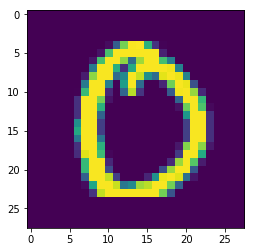
\includegraphics[scale=0.4]{chapter_3_figures/mnist_0.png}
    %\caption{Image}\label{fig:image1}
\end{subfigure}
    \hfill
\begin{subfigure}{.3\linewidth}
    \centering
    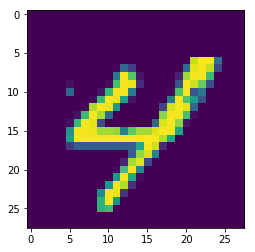
\includegraphics[scale=0.4]{chapter_3_figures/mnist_4.png}
    %\caption{Image}\label{fig:image12}
\end{subfigure}
   \hfill
\begin{subfigure}{.3\linewidth}
    \centering
    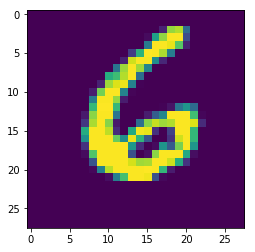
\includegraphics[scale=0.4]{chapter_3_figures/mnist_6.png}
    %\caption{Image}\label{fig:image13}
\end{subfigure}

\bigskip
\begin{subfigure}{.3\linewidth}
    \centering
    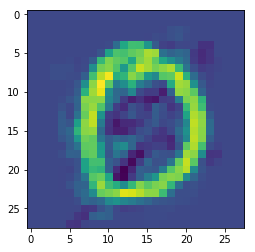
\includegraphics[scale=0.4]{chapter_3_figures/mnist_test_0.png}
    %\caption{Image}\label{fig:image1}
\end{subfigure}
    \hfill
\begin{subfigure}{.3\linewidth}
    \centering
    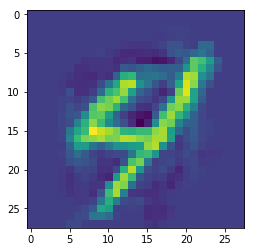
\includegraphics[scale=0.4]{chapter_3_figures/mnist_test_4.png}
    %\caption{Image}\label{fig:image12}
\end{subfigure}
   \hfill
\begin{subfigure}{.3\linewidth}
    \centering
    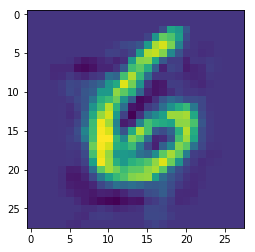
\includegraphics[scale=0.4]{chapter_3_figures/mnist_test_6.png}
    %\caption{Image}\label{fig:image13}
\end{subfigure}
\caption{MNIST digits in the training set recreated by the network. Top row the actual digits, bottom row, the predictive reconstructions.}
\end{figure}
Additionally, the model was also able to recognize and reconstruct previously unseen MNIST digits, albeit with slightly lower fidelity. Nevertheless it is impressive how rapidly and well the network is able to generalize to completely unseen digits.
\newline
\bigskip

\begin{figure}[H]
\centering
\begin{subfigure}{.3\linewidth}
    \centering
    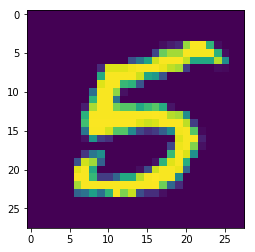
\includegraphics[scale=0.4]{chapter_3_figures/unseen_5.png}
    %\caption{Image}\label{fig:image1}
\end{subfigure}
    \hfill
\begin{subfigure}{.3\linewidth}
    \centering
    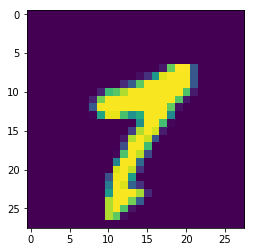
\includegraphics[scale=0.4]{chapter_3_figures/unseen_7.png}
    %\caption{Image}\label{fig:image12}
\end{subfigure}
   \hfill
\begin{subfigure}{.3\linewidth}
    \centering
    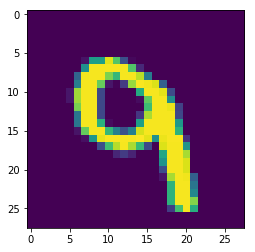
\includegraphics[scale=0.4]{chapter_3_figures/unseen_9.png}
    %\caption{Image}\label{fig:image13}
\end{subfigure}

\bigskip
\begin{subfigure}{.3\linewidth}
    \centering
    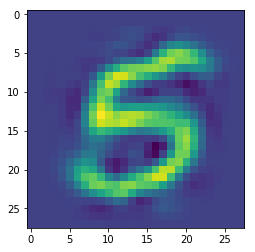
\includegraphics[scale=0.4]{chapter_3_figures/unseen_test_5.png}
    %\caption{Image}\label{fig:image1}
\end{subfigure}
    \hfill
\begin{subfigure}{.3\linewidth}
    \centering
    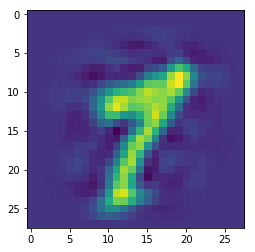
\includegraphics[scale=0.4]{chapter_3_figures/unseen_test_7.png}
    %\caption{Image}\label{fig:image12}
\end{subfigure}
   \hfill
\begin{subfigure}{.3\linewidth}
    \centering
    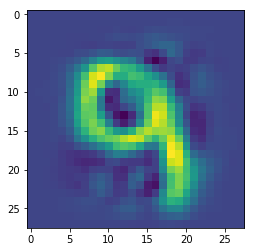
\includegraphics[scale=0.4]{chapter_3_figures/unseen_test_9.png}
    %\caption{Image}\label{fig:image13}
\end{subfigure}
\caption{Unseen MNIST digits in the test set recreated by the network. Top row the actual digits, bottom row, the predictive reconstructions.}
\end{figure}

Since the model is a generative model, it is also able to generalize outside the training set to generate, or `dream', completely unseen digits by sampling from the latent space. Examples are shown below:

\begin{figure}[htb]
\centering
\begin{subfigure}{.3\linewidth}
    \centering
    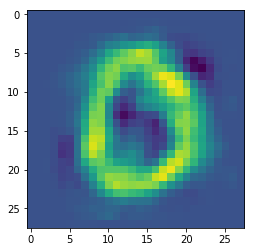
\includegraphics[scale=0.4]{chapter_3_figures/test_test_0.png}
    %\caption{Image}\label{fig:image1}
\end{subfigure}
    \hfill
\begin{subfigure}{.3\linewidth}
    \centering
    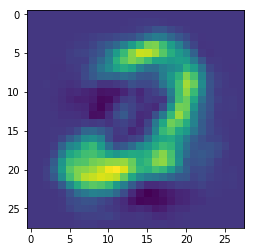
\includegraphics[scale=0.4]{chapter_3_figures/test_test_2.png}
    %\caption{Image}\label{fig:image12}
\end{subfigure}
   \hfill
\begin{subfigure}{.3\linewidth}
    \centering
    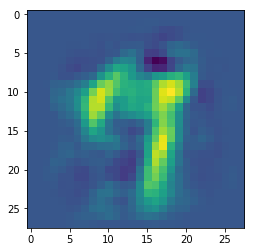
\includegraphics[scale=0.4]{chapter_3_figures/test_test_7.png}
    %\caption{Image}\label{fig:image13}
\end{subfigure}
\caption{Images of hallucinated digits "dreamt" by the network. These were generated by sampling the latent space around the representations of some exemplar digits in the latent space, and then letting the predictive coding network generate its prediction from the chosen latent state.}
\end{figure}

\begin{figure}[H]
\centering
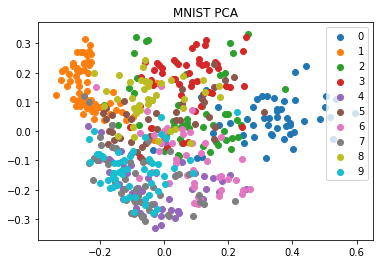
\includegraphics[scale=0.6]{chapter_3_figures/mnist_pca.png}
\caption{A PCA clustering plot of the values of test MNIST digits in the latent space. Even though the 20 dimensional latent space has been reduced down to two, clusters are still visible. For instance, all the 1s are clustered in the top left corner. We thus see that predictive coding appears to be a powerful and fully unsupervised learning algorithm,capable of separating out distinct digits in the latent space, despite not being trained with any label information at all -- and purely on reconstruction.}
\label{PCA_figure}
\end{figure}

Finally, to visualize the latent space, PCA (principal components analysis) was applied to the learned representations in the 20 dimensional latent space to shrink it down to a two dimensional space. It is apparent upon inspection of Figure \ref{PCA_figure} that the latent space, even when shrunk down to two dimensions, does a good job of clustering the MNIST, putting all the 1s in the top left corner, or all the zeros in the middle right. This strongly indicates that the predictive coding model is able to learn the categories of digits despite being trained in an entirely unsupervised way without any knowledge of the true identities of the digits.

We additionally tested the network's capability to reconstruct CIFAR images, which are 32x32 colour images of natural scnes. Our network was the same in the MNIST case except that we used a latent dimension of 50. 

The hierarchical predictive coding CIFAR models are able to learn to reconstruct CIFAR images with impressive fidelity given that they were compressed from a 1024 dimensional image into a 50 dimensional latent state.

\begin{figure}[H]
\centering
\begin{subfigure}{.3\linewidth}
    \centering
    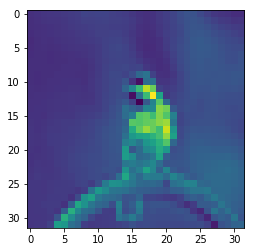
\includegraphics[scale=0.4]{chapter_3_figures/cifar_bird.png}
    %\caption{Image}\label{fig:image1}
\end{subfigure}
    \hfill
\begin{subfigure}{.3\linewidth}
    \centering
    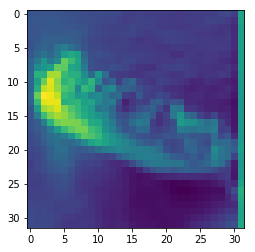
\includegraphics[scale=0.4]{chapter_3_figures/cifar_boat.png}
    %\caption{Image}\label{fig:image12}
\end{subfigure}
   \hfill
\begin{subfigure}{.3\linewidth}
    \centering
    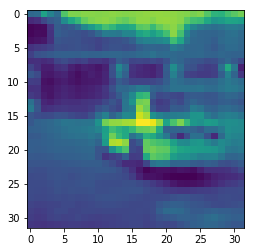
\includegraphics[scale=0.4]{chapter_3_figures/cifar_car.png}
    %\caption{Image}\label{fig:image13}
\end{subfigure}

\bigskip
\begin{subfigure}{.3\linewidth}
    \centering
    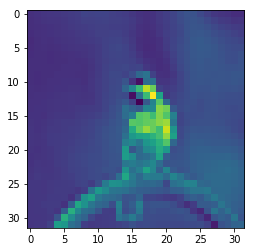
\includegraphics[scale=0.4]{chapter_3_figures/cifar_bird_test.png}
    %\caption{Image}\label{fig:image1}
\end{subfigure}
    \hfill
\begin{subfigure}{.3\linewidth}
    \centering
    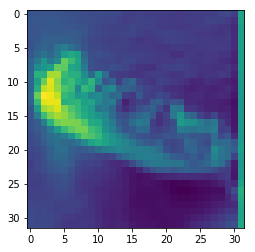
\includegraphics[scale=0.4]{chapter_3_figures/cifar_boat_test.png}
    %\caption{Image}\label{fig:image12}
\end{subfigure}
   \hfill
\begin{subfigure}{.3\linewidth}
    \centering
    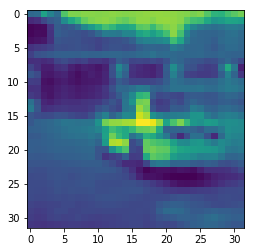
\includegraphics[scale=0.4]{chapter_3_figures/cifar_car_test.png}
    %\caption{Image}\label{fig:image13}
\end{subfigure}
\begin{subfigure}{.3\linewidth}
    \centering
    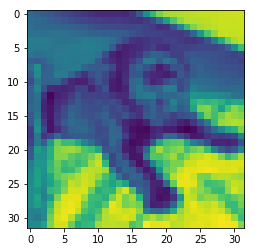
\includegraphics[scale=0.4]{chapter_3_figures/cifar_chimp.png}
    %\caption{Image}\label{fig:image1}
\end{subfigure}
    \hfill
\begin{subfigure}{.3\linewidth}
    \centering
    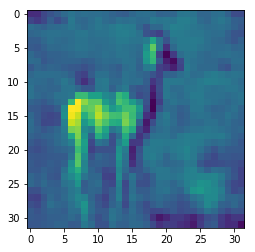
\includegraphics[scale=0.4]{chapter_3_figures/cifar_gazelle.png}
    %\caption{Image}\label{fig:image12}
\end{subfigure}
   \hfill
\begin{subfigure}{.3\linewidth}
    \centering
    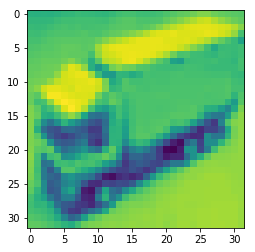
\includegraphics[scale=0.4]{chapter_3_figures/cifar_lorry.png}
    %\caption{Image}\label{fig:image13}
\end{subfigure}

\bigskip
\begin{subfigure}{.3\linewidth}
    \centering
    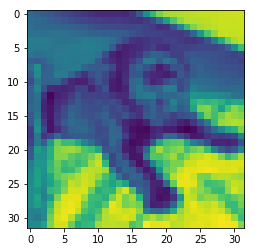
\includegraphics[scale=0.4]{chapter_3_figures/cifar_chimp_test.png}
    %\caption{Image}\label{fig:image1}
\end{subfigure}
    \hfill
\begin{subfigure}{.3\linewidth}
    \centering
    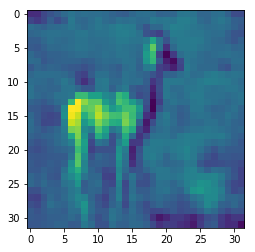
\includegraphics[scale=0.4]{chapter_3_figures/cifar_gazelle_test.png}
    %\caption{Image}\label{fig:image12}
\end{subfigure}
   \hfill
\begin{subfigure}{.3\linewidth}
    \centering
    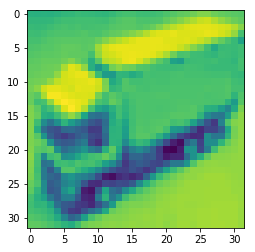
\includegraphics[scale=0.4]{chapter_3_figures/cifar_lorry_test.png}
    %\caption{Image}\label{fig:image13}
\end{subfigure}
\caption{Test set CIFAR digits reconstructed by the network. The first of the two lines is the image and the second is the reconstruction. The network is extremely good at reconstructing CIFAR images.}
\end{figure}

Importantly, due to having learnt a latent space, we are able to \emph{interpolate} between images, and thus investigate the properties of the learnt latent space. To interpolate, we begin with two images $o_1$ and $o_2$ and take the difference vector in the latent space $\epsilon = f(o_2) - f(o_1)$ where $f$ is the encoder function. Then, we step in the latent space by a constant $\alpha$ and decode such that $\hat{o} = g(f(o_2) + \alpha \epsilon)$ where $g$ is the decoding function. We stepped in increments of $\alpha = 0.1$. Below we can see the network smoothly interpolating between an image of a horse and a cat. We see that the predictive coding network appears to naturally learn a smooth latent space, allowing for generalization to unseen images and smooth interpolation between classes in the latent space.
\begin{figure}[H]
\centering
\begin{subfigure}{.3\linewidth}
    \centering
    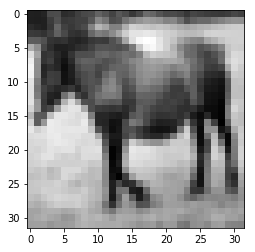
\includegraphics[scale=0.4]{chapter_3_figures/interp_2.png}
    %\caption{Image}\label{fig:image1}
\end{subfigure}
    \hfill
\begin{subfigure}{.3\linewidth}
    \centering
    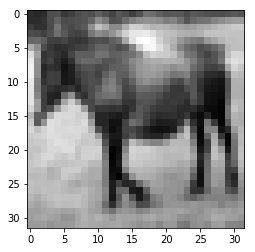
\includegraphics[scale=0.4]{chapter_3_figures/interp_3.png}
    %\caption{Image}\label{fig:image12}
\end{subfigure}
   \hfill
\begin{subfigure}{.3\linewidth}
    \centering
    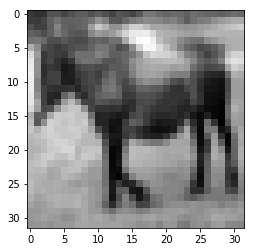
\includegraphics[scale=0.4]{chapter_3_figures/interp4.png}
    %\caption{Image}\label{fig:image13}
\end{subfigure}

\bigskip
\begin{subfigure}{.3\linewidth}
    \centering
    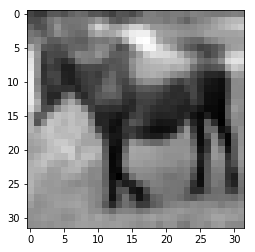
\includegraphics[scale=0.4]{chapter_3_figures/interp5.png}
    %\caption{Image}\label{fig:image1}
\end{subfigure}
    \hfill
\begin{subfigure}{.3\linewidth}
    \centering
    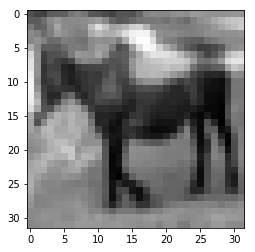
\includegraphics[scale=0.4]{chapter_3_figures/interp6.png}
    %\caption{Image}\label{fig:image12}
\end{subfigure}
   \hfill
\begin{subfigure}{.3\linewidth}
    \centering
    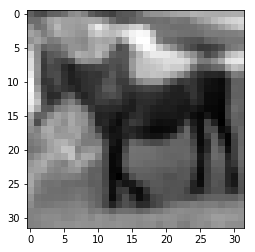
\includegraphics[scale=0.4]{chapter_3_figures/interp7.png}
    %\caption{Image}\label{fig:image13}
\end{subfigure}
\begin{subfigure}{.3\linewidth}
    \centering
    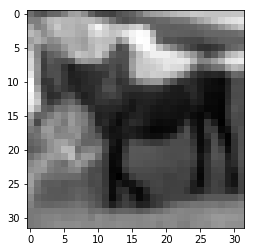
\includegraphics[scale=0.4]{chapter_3_figures/interp8.png}
    %\caption{Image}\label{fig:image1}
\end{subfigure}
    \hfill
\begin{subfigure}{.3\linewidth}
    \centering
    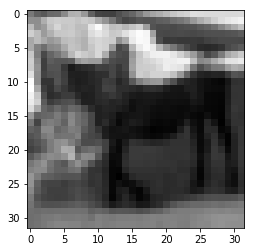
\includegraphics[scale=0.4]{chapter_3_figures/interp9.png}
    %\caption{Image}\label{fig:image12}
\end{subfigure}
   \hfill
\begin{subfigure}{.3\linewidth}
    \centering
    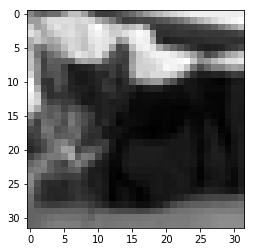
\includegraphics[scale=0.4]{chapter_3_figures/interp10.png}
    %\caption{Image}\label{fig:image13}
\end{subfigure}
\caption{The CIFAR model interpolating between a horse and a cat. Read the images left to right top to bottom - like text. The interpolation is done by stepping in the latent space from the representation of the first image in the direction of the second until it is reached.}
\end{figure}

\subsection{Dynamical Predictive coding}

While so far,  we have only considered the modelling just a single static stimulus $o$. However, the data the brain receives comes in temporal sequences $\bar{o} = [o_1, o_2 \dots ] $. To model such temporal sequences, it is often useful to split the latent variables into \emph{states}, which can vary with time, and \emph{parameters} which cannot. In the case of sequences, instead of minimizing the variational free energy, we must instead minimize the \emph{free action} $\bar{\mathcal{F}}$, which is simply the path integral of the variational free energy through time:
\begin{align*}
    \mu^* &= \underset{\mu}{argmin} \, \, \bar{\mathcal{F}} \\
    \bar{\mathcal{F}}  &= \int dt \mathcal{F}_t \\
    \mathcal{F}_t &= \KL \left[ q(x_t | o_t; \phi)|| p(o_t, x_t | x_{t-1}) \right] \numberthis
\end{align*}

While there are numerous methods to handle sequence data, one influential and elegant approach \citep{friston2008DEM,friston2008hierarchical,friston2010generalised} is to represent temporal data in terms of \emph{generalized coordinates of motion}. These coordinates represent not just the immediate observation state, but all the temporal derivatives of the observation. For instance, suppose that the brain represents beliefs about the position of an object. Under a generalized coordinate model, it would also represent beliefs about the velocity (first time derivative), acceleration (second time derivative), jerk (third time derivative) and so on. All these time derivative beliefs are concatenated to form a generalized state. The key insight into this dynamical formulation is, that when written in such a way, many of the mathematical difficulties in handling sequences disappear, leaving relatively straightforward and simple variational filtering algorithms which natively handle smoothly changing sequences. For instance, we maintain a coherent concept of a stationary state, since we can define it as one in which none of the time derivatives are changing. This allows the variational inference procedure to track a moving target by representing it as a steady state in a moving frame of reference.

Because the generalised coordinates are notationally awkward, we will be very explicit in the following. We denote the time derivatives of the generalized coordinate using a $'$, so $\mu'$ is the belief about the velocity of the $\mu$, just as $\mu$ is the belief about the `position' about the $\mu$. A key point of confusion is that there is also a `real' velocity of $\mu$, which we denote $\dot{\mu}$, which represents how the belief in $\mu$ actually changes over time. Importantly, this is not necessarily the same as the belief in the velocity: $\dot{\mu} \neq \mu'$,except at the equilibrium state. Intuitively, this makes sense as at equilibrium (mimimum of the free action, and thus perfect inference), our belief about the velocity of mu $\mu'$ and the `real' velocity perfectly match. Away from equilibrium, our inference is not perfect so they do not necessarily match. We denote the generalized coordinate representation of a state $\tilde{\mu}$ as simply a vector of each of the beliefs about the time derivatives $\tilde{\mu} = [\mu, \mu', \mu'', \mu''' \dots]$. We also define the operator $\mathcal{D}$ which maps each element of the generalised coordinate to its time derivative i.e. $\mathcal{D}\mu = \mu', \mathcal{D}\tilde{\mu} = [\mu', \mu'', \mu''',\mu'''' \dots]$. With this notation, we can define a dynamical generative model using generalized coordinates. Crucially, we assume that the noise $\omega$ in the generative model is not white noise, but is colored, so it has non-zero autocorrelation and can be differentiated. Effectively, colored noise allows one to model relatively slowly (not infinitely fast) exogenous forces on the system. For more information on colored noise vs white noise see \citep{friston2008DEM,yuan2012beyond}. With this assumption we can obtain a generative model in generalized coordinates of motion by simply differentiating the original model.
\begin{align*}
    o &= f(x) + \omega_o  && x = g(\bar{x}) + \omega_x \\
    o' &= f'(x)x' + \omega_o' && x' = g'(\bar{x})x' + \omega_x'\\
    o'' &= f'(x)x'' + \omega_o'' && x'' = g'(\bar{x})x'' + \omega_x'' \\
    &\dots && \dots \numberthis
\end{align*}
Where we have applied a local linearisation assumption \citep{friston2008DEM} which drops the cross terms in the derivatives. We can write these generative models more compactly in generalized coordinates.
\begin{align*}
    \tilde{o} = \tilde{f}(\tilde{x}) + \tilde{\omega}_o && \tilde{x} = \tilde{g}(\tilde{\bar{x}}) + \tilde{\omega}_x \numberthis
\end{align*}
which, written probabilistically is $p(\tilde{o},\tilde{x}) = p(\tilde{o} | \tilde{x})p(\tilde{x})$. It has been shown \citep{friston2008DEM} that the optimal (equilibrium) solution to this free action is the following stochastic differential equation,
\begin{align*}
    \label{dynamical_mu_integration}
    \dot{\tilde{\mu}} = \mathcal{D}\tilde{\mu} + \frac{\partial \mathbb{E}_{q(\tilde{x} | \tilde{o}; \tilde{\mu})}[\ln p(\tilde{o}, \tilde{x})]}{\partial \tilde{\mu}} + \tilde{\omega} \numberthis
\end{align*}
Where $\tilde{\omega}$ is the generalized noise at all orders of motion. Intuitively, this is because when $\frac{\partial \mathbb{E}_{q(x | o; \mu)}[\ln p(\tilde{o}, \tilde{x})]}{\partial \mu} = 0$ then $\dot{\tilde{\mu}} = \mathcal{D}\tilde{\mu}$, or that the `real' change in the variable is precisely equal to the expected change. This equilibrium is a dynamical equilibrium which moves over time, but precisely in line with the beliefs $\mu'$. This allows the system to track a dynamically moving optimal solution precisely, and the generalized coordinates let us capture this motion while retaining the static analytical approach of an equilibrium solution, which would otherwise necessarily preclude motion. There are multiple options to turn this result into a variational inference algorithm. Note, the above equation makes no assumptions about the form of variational density or the generative model, and thus allows multimodal or nonparametric distributions to be represented. For instance, the above equation (Equation \ref{dynamical_mu_integration}) could be integrated numerically by a number of particles in parallel, thus leading to a generalization of particle filtering \citep{friston2008variational}. Alternatively, a fixed Gaussian form for the variational density can be assumed, using the Laplace approximation. In this case, we obtain a very similar algorithm to predictive coding as before, but using generalized coordinates of motion. In the latter case, we can write out the free energy as,
\begin{align*}
    \mathcal{F}_t &= \ln p(\tilde{o} | \tilde{x})p(\tilde{x}) \\
    &\propto \tilde{\Sigma}^{-1}_o \tilde{\epsilon}_o^2 + \tilde{\Sigma}^{-1}_x \tilde{\epsilon}_x^2  \numberthis
\end{align*}
Where $\tilde{\epsilon}_o =  \tilde{o} - \tilde{f}(\tilde{x})$ and $\tilde{\epsilon}_x =  \tilde{o} - \tilde{g}(\tilde{\bar{x}})$. Moreover, the generalized precisions $\tilde{\Sigma}^{-1}$ not only encode the covariance between individual elements of the data or latent space at each order, but also the correlations between generalized orders themselves. Since we are using a unimodal (Gaussian) approximation, instead of integrating the stochastic differential equations of multiple particles, we instead only need to integrate the deterministic differential equation of the mode of the free energy,
\begin{align*}
    \dot{\tilde{\mu}} = \mathcal{D}\tilde{\mu} - \tilde{\Sigma}^{-1}_o \tilde{\epsilon}_o - \tilde{\Sigma}^{-1}_x \tilde{\epsilon}_x \numberthis
\end{align*}
which cashes out in a scheme very similar to standard predictive coding (compare to Equation \ref{PC_hierarchical_mu}), but in generalized coordinates of motion. The only difference is the $\mathcal{D}\tilde{\mu}$ term which links the orders of motion together. This term can be intuitively understood as providing the `prior motion' while the prediction errors provide `the force' terms. To make this clearer, let's take a concrete physical analogy where $\mu$ is the position of some object and $\mu'$ is the expected velocity. Moreover, the object is subject to forces $\tilde{\Sigma}^{-1}_o \tilde{\epsilon}_o + \tilde{\Sigma}^{-1}_x \tilde{\epsilon}_x$ which instantaneously affect its position. Now, the total change in position $\dot{\tilde{\mu}}$ can be thought of as first taking the change in position due to the intrinsic velocity of the object $\mathcal{D}\mu$ and adding that on to the extrinsic changes due to the various exogenous forces. 

Things get more complex when we consider a model which has both dynamical and hierarchical components where there are interactions between them. This we call a full-construct model following the lead of this tutorial \citep*{buckley2017free}. In a full construct model there is a dynamical hierarchy of levels where it is assumed that each dynamical order is only able to affect the level below:

\begin{flalign*}
o &= f(\mu ;\theta) \\
\mu &= f'(\mu' ; \theta')\\
\mu' &= f'(\mu'' ; \theta'') \\
... \numberthis
\end{flalign*}

Similarly, there is an simultaneously a hierarchy of levels, where each level is assumed to be predicted by the level above it:
\begin{flalign*}
o &= g(\mu_0 ; \theta_0) \\
\mu_0 &= g'(\mu_1 ; \theta_1) \\
\mu_1 &= g'(\mu_2 ; \theta_2) \\
\mu2 &= g'(\mu_3 ; \theta_3) \\
... \numberthis
\end{flalign*}
Therefore, each node in the lattice of hierarchical and dynamic hierarchies is influenced by two separate predictions - the dynamical prediction going from higher dynamical orders to lower, and the hierarchical prediction propagating from higher levels of the hierarchy to lower ones. Thus, a single state of a cause-unit $\mu_i^n$, where $i$ is the level of the hierarchy, and $n$ is the dynamical order, is defined to be:
\begin{align*}
\mu_i^n = f(\mu_i^{n+1} ; \theta_i^{n+1}) + g(\mu_{i+1}^n ; \theta_{i+1}^n) \numberthis
\end{align*}

This means that the variational free energy must sum over both dynamical and hierarchical prediction errors, such that:
\begin{align*}
\mathcal{F} = \sum_i \sum_n {\Sigma^n_i}^{-1} {\epsilon_i^n}^2 \numberthis
\end{align*}

And that additionally the updates for the representation-units and the weights must take this into account. The revised update rules are presented below:
\begin{flalign*}
\frac{d\mu_i^n}{dt} &= \Sigma_{n+1}^{-1} \epsilon_i^{n+1} \frac{df}{d\mu_i^n}\theta_i^{n+1} + \Sigma_n^{-1} \epsilon_i^n + \Sigma_{i-1}^{-1} \epsilon_{i-1}^n \frac{dg}{d\mu_i^n} \theta_{i-1}^n + \Sigma_i^{-1} \epsilon_i^n \numberthis
\end{flalign*}

And for the weights the update rule thus becomes:
\begin{align*}
\frac{d\theta_i^n}{dt} = \Sigma_i^n \epsilon_i^n (\frac{df}{d\theta_i^n}{\mu_i^{n+1}}^T + \frac{dg}{d\theta_i^n} {\mu_{i+1}^n}^T) \numberthis
\end{align*}

These rules appear somewhat more complicated than the corresponding rules in the static case. Nevertheless they only incur a linear (in the order of generalized coordinates considered) additional computational cost.

Preliminary dynamical and full construct models were implemented and tested on simple stimuli. The first task the dynamical models were tested on was predicting a sine wave. This is the perfect toy-task since sine waves have analytic derivatives to any infinite degree. We used a dynamical model which represented three orders of generalized motion. The model was trained to predict a sine wave autoregressively and it's first two temporal derivatives. The model rapidly learned to predict the sine wave, as can be seen from the training graphs below. However, there was a consistent phase-error in the predictions it made, which could have been caused by the rapid rate of change of the sine-wave observations.

\begin{figure}[H]
\centering
\begin{subfigure}{.3\linewidth}
    \centering
    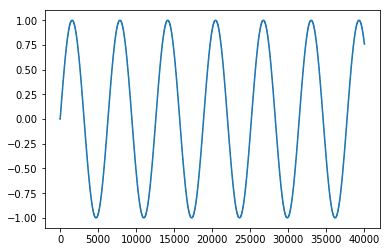
\includegraphics[scale=0.5]{chapter_3_figures/dynamics_sine_wave_phi.png}
    \caption{Incomding sense data - i.e. a sine wave}
\end{subfigure}
    \hfill
\begin{subfigure}{.3\linewidth}
    \centering
    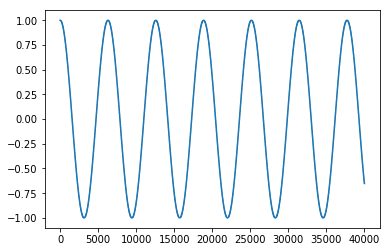
\includegraphics[scale=0.5]{chapter_3_figures/dynamics_sine_wave_phidot.png}
    \caption{First derivative of the incoming sense data}
\end{subfigure}

\bigskip
\begin{subfigure}{.3\linewidth}
    \centering
    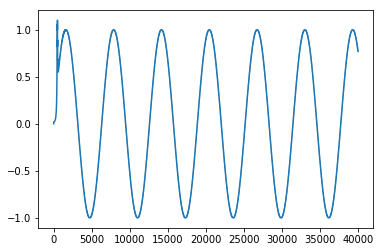
\includegraphics[scale=0.5]{chapter_3_figures/dynamics_sine_wave_predphi.png}
    \caption{Predicted incoming sense data}
\end{subfigure}
    \hfill
\begin{subfigure}{.3\linewidth}
    \centering
    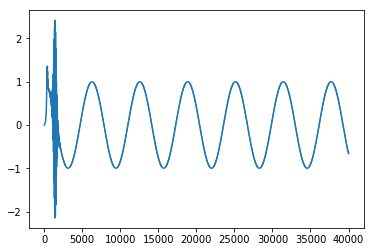
\includegraphics[scale=0.5]{chapter_3_figures/dynamics_sine_wave_pred_phidot.png}
    \caption{Prediction temporal derivative of the incoming sense data}
\end{subfigure}

\bigskip
  
\begin{subfigure}{.3\linewidth}
    \centering
    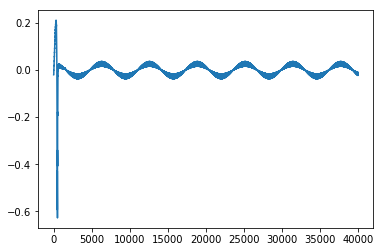
\includegraphics[scale=0.5]{chapter_3_figures/dynamics_sine_wave_ez1.png}
    \caption{Prediction error at the first dynamical level}
\end{subfigure}
\hfill
\begin{subfigure}{.3\linewidth}
    \centering
    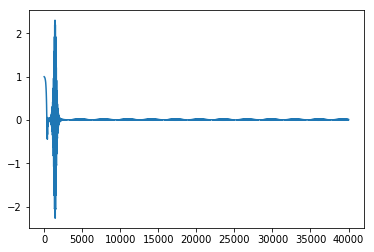
\includegraphics[scale=0.5]{chapter_3_figures/dynamics_sine_wave_ez2.png}
    \caption{Prediction error at the second dynamical level}
\end{subfigure}
    
\bigskip
\begin{subfigure}{.3\linewidth}
    \centering
    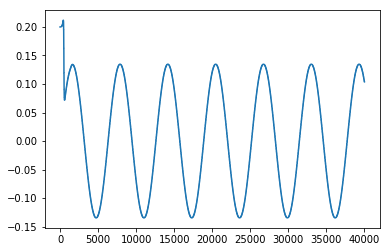
\includegraphics[scale=0.5]{chapter_3_figures/dynamics_sine_wave_thetaz1.png}
    \caption{Acitvation of representation units at the first dynamical level}
\end{subfigure}
   \hfill
\begin{subfigure}{.3\linewidth}
    \centering
    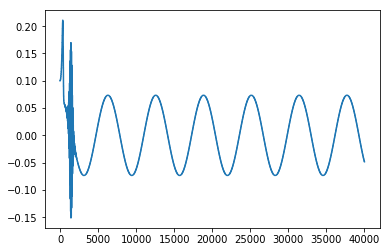
\includegraphics[scale=0.5]{chapter_3_figures/dynamics_sine_wave_theta_z2.png}
    \caption{Activation of the representation units at the second dynamical level}\label{fig:image13}
\end{subfigure}
\caption{Prediction errors and prediction for simple toy dynamical models. The task of the dynamical predictive coding model is to learn to predict a sinewave using only the first two dynamical orders -- so including position, velocity, and acceleration. The model starts from randomly initialized parameters. We see that the model very quickly learns to match the incoming sine wave observations with only minimal error at the beginning.}
\end{figure}

The dynamical model does not only work with sine waves. The model was also tested on more jerky waveforms sawtooth waves. In this case a two layer linear dynamical model was used which learned to predict the sawtooth wave and its first temporal derivative. The model predicts the wave very successfully, including the temporal derivative, although there it is a little less successful. Once again there is a persistent patterned prediction error, likely caused by the lag time between the models predictions and the the observations it receives. 
\begin{figure}[H]
\centering
\begin{subfigure}{.3\linewidth}
    \centering
    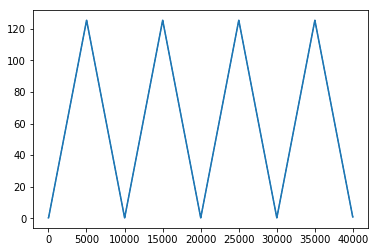
\includegraphics[scale=0.4]{chapter_3_figures/sawtooth_phi.png}
    \caption{Incomding sense data - the sawtooth wave}
\end{subfigure}
    \hfill
\begin{subfigure}{.3\linewidth}
    \centering
    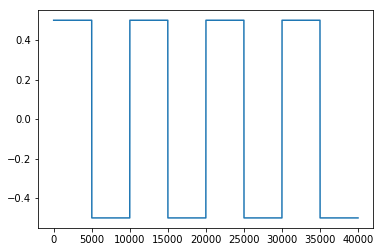
\includegraphics[scale=0.4]{chapter_3_figures/sawtooth_phidot.png}
    \caption{First derivative of the incoming sense data}
\end{subfigure}
\hfill
\begin{subfigure}{.3\linewidth}
    \centering
    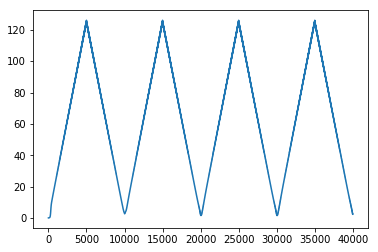
\includegraphics[scale=0.4]{chapter_3_figures/sawtooth_pred_phi.png}
    \caption{Predicted incoming sense data}
\end{subfigure}

\bigskip
\begin{subfigure}{.3\linewidth}
    \centering
    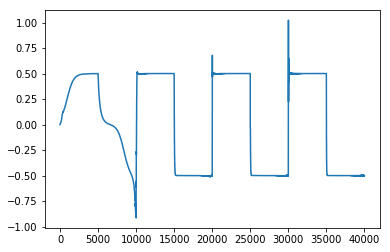
\includegraphics[scale=0.4]{chapter_3_figures/sawtooth_predphidot.png}
    \caption{Prediction temporal derivative of the incoming sense data}
\end{subfigure}
\hfill
\begin{subfigure}{.3\linewidth}
    \centering
    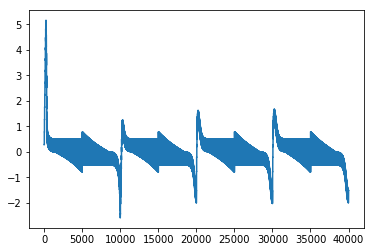
\includegraphics[scale=0.4]{chapter_3_figures/sawtooth_pe1.png}
    \caption{Prediction error at the first dynamical level}
\end{subfigure}
\hfill
\begin{subfigure}{.3\linewidth}
    \centering
    \includegraphics[scale=0.4]{chapter_3_figures/sawtooth_pe2.png}
    \caption{Prediction error at the second dynamical level}
\end{subfigure}
    
\bigskip
\begin{subfigure}{.3\linewidth}
    \centering
    \includegraphics[scale=0.4]{chapter_3_figures/sawtooth_mu1.png}
    \caption{Activation of representation units at the first dynamical level}
\end{subfigure}
   \hfill
\begin{subfigure}{.3\linewidth}
    \centering
    \includegraphics[scale=0.4]{chapter_3_figures/sawtooth_mu2.png}
    \caption{Activation of the representation units at the second dynamical level}
\end{subfigure}
\caption{Dynamical models tested on more challenging sawtooth and square wave inputs. The model was randomly initialized and only modelled the first two dynamical orders (so position, velocity, accelearation). Apart from a brief initial period of uncertainty, the model rapidly learned to predict these more challenging wave shapes.}
\end{figure}


We can also train `full-construct' models on dynamical stimuli. Here we used a model with two hierarchical layers and three dynamical layers and was trained autoregressively to predict a sine-wave. Training was `online' with a learning rate of $0.01$. The generative model parameters $\theta$ were updated initialized randomly and updated each epoch. For every `tick' of the sine wave, the variational parameters $\mu$ were updated for 100 steps. Training graphs are shown below:

\begin{figure}[H]
\centering
\begin{subfigure}{.3\linewidth}
    \centering
    \includegraphics[scale=0.35]{chapter_3_figures/fc_phi.png}
    \caption{Incomding sense data - Sine wave}
\end{subfigure}
    \hfill
\begin{subfigure}{.3\linewidth}
    \centering
    \includegraphics[scale=0.35]{chapter_3_figures/fc_phidot.png}
    \caption{First derivative of the sense-data}
\end{subfigure}
\hfill
\begin{subfigure}{.3\linewidth}
    \centering
    \includegraphics[scale=0.35]{chapter_3_figures/fc_phidotdot.png}
    \caption{Predicted incoming sense data}
\end{subfigure}
\bigskip

\begin{subfigure}{.3\linewidth}
    \centering
    \includegraphics[scale=0.35]{chapter_3_figures/fc_predphi.png}
    \caption{The models' prediction of the incomign sense data}%\label{fig:image12}
\end{subfigure}
\hfill
\begin{subfigure}{.3\linewidth}
    \centering
    \includegraphics[scale=0.35]{chapter_3_figures/fc_predphidot.png}
    \caption{The models' prediction of the first derivative of the incoming sense-data}%\label{fig:image13}
\end{subfigure}
\hfill
\begin{subfigure}{.3\linewidth}
    \centering
    \includegraphics[scale=0.35]{chapter_3_figures/fc_predphidotdot.png}
    \caption{the models' prediction of the second derivative of the incoming sense-data}%\label{fig:image1}
\end{subfigure}
    
\bigskip
\begin{subfigure}{.3\linewidth}
    \centering
    \includegraphics[scale=0.35]{chapter_3_figures/fc_ez1.png}
    \caption{The prediction error at the first hierarcical layer}%\label{fig:image12}
\end{subfigure}
   \hfill
\begin{subfigure}{.3\linewidth}
    \centering
    \includegraphics[scale=0.35]{chapter_3_figures/fc_ez2.png}
    \caption{The prediction error at the second hierarcical layer}%\label{fig:image13}
\end{subfigure}
\hfill
\begin{subfigure}{.3\linewidth}
    \centering
    \includegraphics[scale=0.35]{chapter_3_figures/fc_ew11.png}
    \caption{The prediction error at the first dynamical layer}%\label{fig:image12}
\end{subfigure}
   \hfill
%\begin{subfigure}{.3\linewidth}
%    \centering
%    \includegraphics[scale=0.35]{chapter_3_figures/fc_ew12.png}
%    \caption{The prediction error at the second dynamical layer}\label{fig:image13}
%\end{subfigure}
\caption{The training graphs of the full construct model. It can successfully predict the first three temporal derivatives of a sine wave, and also minimise prediction error up to multiple hierarchical layers. The full construct model was randomly initialized, and learnt both parameters and inferred states purely online -- thus achieving a `double deconvolution' \citep{friston2008DEM}.}
\end{figure}

The top two rows of graphs show the incoming sense data and the first two temporal derivatives of the sense-data. The next two rows show the prediction errors over time for various levels of the hierarchy. The full construct model appears a bit less stable and successful than the simple dynamical model, likely because it is much more complex and has many more moving parts. Nevertheless it manages to learn the sine wave shapes relatively faithfully and does also manage to rapidly reduce the prediction error over time. Moreover these sorts of tasks do not really play well to the strength of the full-construct model since the input data (the sine wave) contains no suitable hierarchical structure for the higher levels to model. It seems likely that as these models are scaled up to more challenging tasks, the greater expressivity and power of the full-construct models will become more apparent. So far, we have only experimented with `full-construct' models on simple toy tasks such as sine waves. An interesting avenue for future would work be experimenting as to whether full construct models could be scaled up to handle challenging machine learning tasks dealing with sequential data such as video prediction. While preditive coding networks have been proposed for this task \citep{lotter2016deep}, none to our knowledge have explicitly utilized generalized coordinates in any capacity.

\section{Predictive Coding and Kalman Filtering}

A key intuition behind the utility of predictive coding is that it naturally handles \emph{filtering} tasks. Filtering tasks require constant updates of a moving state estimate given sequences of new data. Effectively, filtering is the task of learning and inferring movements in the hidden state of the world from changing input \emph{sequences} -- as opposed to the usual machine learning task of inferring hidden states (such as labels) from single static inputs. Importantly the core task faced by much of the brain is fundamentally one of filtering, since the inputs the brain receives are actually temporally extended sequences, rather than static flashes. For instance, in vision the task of the brain is not to categorize static images but rather to infer the state of, and ultimately interact with, a smoothly changing external world situated in continuous time. Moreover, it is known that the brain takes substantial advantage of the additional information given by integrating sequences over time such as optical flow \citep{gibson2002theory} and active motion to explore different angles on a given scene \citep{henderson2017gaze}.

If, as we generally assume throughout the thesis, that the brain is fundamentally a (Bayesian) inference machine, then the core task of the brain must be \emph{Bayesian Filtering} instead of static Bayesian inference \citep{sarkka2013Bayesian}. Bayesian filtering is mathematically somewhat more involved, due to the need to perform inference over sequences instead of single data-points, but there are a wide variety of algorithms in the literature which perform Bayesian filtering, often highly effectively \citep{kutschireiter2018nonlinear,kutschireiter2020hitchhiker}. Mathematically, we can formalize the filtering problem as follows \citep*{jaswinskistochastic,stengel1994optimal}. We have an estimated state $\hat{x}_t$, and some model of how the world evolves (the dynamics model): $\hat{x}_{t+1} = f(\hat{x}_t)$. We also receive observations $o$, and you have some model of how the observations depend on the estimated state (the observation model): $o = g(\hat{x}_t)$. The task, then, is to compute $p(\hat{x}_{t+1} | \hat{x}_t, o_{1...t})$. In the general nonlinear case, this calculation is analytically intractable and extremely expensive to compute exactly. Some form of approximate solution is required. Two forms of approximation are generally used. The first is to approximate the model - such as by assuming linearity of the dynamics and observation models.  

The second method is to approximate the posterior -- usually with a set of samples (or particles). This approach is taken by the class of particle filtering algorithms which track the changing posterior by propagating the particles through the dynamics and then resampling based upon updated measurement information \citep*{arulampalam2002tutorial,gordon1993novel}. This approach can handle general nonlinear filtering cases, but suffers strongly from the curse of dimensionality. If the state-space is high-dimensional the number of particles required for a good approximation grows rapidly \citep*{doucet2000sequential}.Moreover, there has been some fascinating work on implementing particle filtering methods in neural circuitry \citep*{kutschireiter2015neural}, as well as speculation about whether perhaps the brain may utilize particle or sampling methods for inference instead of variational ones \citep{sanborn2016Bayesian}.

Nevertheless, here we focus primarily on approximate variational approaches to inference. Specifically, we first demonstrate that predictive coding is naturally a filtering algorithm -- perhaps more naturally than one applied to static datasets. The only change to the algorithm is simply \emph{what} is predicted. If predictive coding is set up so as to predict the \emph{next} input \citep{mumford1992computational,clark_whatever_2013}, which is highly plausible in the brain, then it can perform variational Bayesian filtering. In this section, we explore this predictive coding filtering algorithm and show, crucially, that in the linear case it becomes a variant of Kalman filtering -- a fundamental and ubiquitous algorithm in classical control \citep{kalman1960contributions,kalman1960new}. Moreover, in the nonlinear case, predictive coding becomes a variant of extended Kalman filtering \citep{ollivier2019extended}. The Kalman Filter solves the general filtering problem by making two simplifying assumptions. The first is that both the dynamics model and the observation model are linear. The second assumption is that noise entering the system is white and Gaussian. This makes both the prior and likelihoods Gaussian. Since the Gaussian distribution is a conjugate prior to itself, this induces a Gaussian posterior, which can then serve as the prior in the next timestep. Since both prior and posterior are Gaussian, filtering can continue recursively for any number of time-steps without the posterior growing in complexity and becoming intractable. The Kalman filter is the Bayes-optimal solution provided that the assumptions of linear models and white Gaussian noise are met \citep*{kalman1960new}. The Kalman Filter, due to its simplicity and utility is widely used in engineering, time-series analysis, aeronautics, and economics \citep*{grewal2010applications,leondes1970theory,schneider1988analytical,harvey1990forecasting}.

Since predictive coding possesses several neurophysiologically realistic process theories \citep{bastos2012canonical}, this correspondence provides an avenue for a biologically plausible implementation of Kalman filtering in the brain. There is substantial evidence that the brain is capable of Bayes-optimal integration of noisy measurements, and is apparently in possession of robust forward models both in perception \citep*{zago2008internal,simoncelli2009optimal} and motor control\citep*{munuera2009optimal, gold2003influence,todorov2004optimality}. \citet*{de2013kalman} have even shown that a Kalman filter successfully fits psychomotor data on visually guided saccades and smooth pursuit movement, although they remain agnostic on how it may be implemented in the brain. We demonstrate, however, a clear mathematical link of the relationship between Kalman filtering and predictive coding, allowing us first to use results from Kalman filtering to understand the performance of predictive coding algorithms, and second enabling us to utilize the process theories of predictive coding to understand how the brain may perform crucial filtering tasks.

First, we reveal the precise relationship between Kalman filtering and predictive coding -- namely that both optimize the same Bayesian objective, which is convex in the linear case. However, the Kalman filter solves the optimization problem analytically, thus giving rise to its algebraic complexities and especially the highly neurobiologically implausible Kalman gain matrix. Predictive coding, on the other hand, solves the objective through a process of gradient descent on the sufficient statistics of the variational distribution, thereby obtaining biologically plausible Hebbian update rules. Additionally, the fully Bayesian perspective granted by predictive coding also allows us to perform learning of the generative model -- i.e. learning the coefficients of the dynamics and likelihood matrices -- which allows us to handle cases where the model of the world is unknown, in contrast to traditional Kalman filtering which assumes accurate (and linear) dynamics and observation models of the world. While the close relationship between Kalman filtering and (linear) predictive coding has been hinted at before \citep{friston2005theory,friston2008hierarchical}, there it is claimed that predictive coding is `equivalent' to Kalman filtering -- which is not case except insofar as the two algorithms optimize the same objective. \citet{baltieri2020kalman} provide side by side comparisons of the update rules for predictive coding and Kalman filtering, but do not go beyond this superficial analysis to uncover the precise relationship between them. 

Secondly, we directly compare the performance of the Kalman filter and our predictive coding algorithm on a simplified location tracking task -- which the Kalman filter excels at. We show that despite the predictive coding algorithm performing a gradient descent instead of an analytical solution, it performs comparably with the Kalman filter and, due to the convexity of the underlying optimization problem, requires very few iterations to converge. This rapid convergence is important, since the brain is heavily time-constrained in its inferences -- choices often must be made fast. Secondly, we demonstrate that the learning rules for the likelihood and dynamics matrices allow us to perform online tracking even when the model is completely unknown. We only show that this is the case for the dynamics, however, as learning does not perform well with an unknown observation model. We hypothesize that this is due to the ill-posedness of the resulting optimization problem.

\subsection{The Kalman Filter}
The Kalman Filter is defined upon the following linear state-space \footnote{For simplicity, the model is presented in discrete time. The continuous time analogue of the Kalman filter is the Kalman-Bucy filter \citep*{kalman1961new}. Generalization of this scheme to continuous time is an avenue for future work.}
\begin{flalign*}
    x_{t+1} &= Ax_t + Bu_t + \omega & \\
    o_{t+1} &= Cx_{t+1} + z_t \numberthis
\end{flalign*}
Where $x_t$ represents the hidden or internal state at time t. $u_t$ is the control - or known inputs to the system - at time t. Matrices $A$,$B$, and $C$ parametrize the linear dynamics or observation models, and $\omega$ and $z$ are both zero-mean white noise Gaussian processes with covariance $\Sigma_\omega$ and $\Sigma_z$, respectively. Since the posterior $p(x_{t+1}|o_{1...t}, x_{t})$ is Gaussian, it can be represented by its two sufficient statistics -- the mean $\mu$ and covariance matrix $\Sigma_x$.

Kalman filtering proceeds by first `projecting' forward the current estimates according to the dynamics model. Then these estimates are `corrected' by new sensory data. The Kalman filtering equations are as follows:
\newline
\textbf{Projection}
\begin{flalign*}
    & \hat{\mu}_{t+1} = A\mu_t + Bu_t  &\\
    & \hat{\Sigma}_x(t+1) = A\Sigma_x(t) A^T + \Sigma_\omega \numberthis
\end{flalign*}
\textbf{Correction}
\begin{flalign*}
    & \mu_{t+1} = \hat{\mu}_{t+1} + K(o_{t+1} - C\hat{\mu}_{t+1}) & \\
    & \Sigma_x(t+1) = (I - K)\hat{\Sigma}_x(t+1) \\
    & K = \hat{\Sigma}_x(t+1)C^T[C\hat{\Sigma}_x(t+1)C^T + \Sigma_z]^{-1} \numberthis
\end{flalign*}

Where $\mu_t$ and $\Sigma_x(t)$ are the mean and variance of the estimate of the state $x$ at time t, and $K$ is the Kalman gain matrix. Although these update rules provide an analytically exact solution to the filtering problem, the complicated linear algebra expressions, especially that for the Kalman gain matrix $K$, make it hard to see how such equations could be implemented directly in the brain. 

Importantly, these Kalman filtering equations can be derived directly from Bayes' rule. The mean of the posterior distribution is also the MAP (maximum-a-posteriori) point, since a Gaussian distribution is unimodal. Thus, to estimate the new mean, we simply have to estimate,
\begin{flalign*}
    \label{KF_MAP}
     &\underset{\hat{x}_{t+1}}{arg max} \, \,  p(\hat{x}_{t+1} | o_{t+1}, \hat{x}_t) \propto \underset{\hat{x}_{t+1}}{argmax} \, p(o_{t+1} |\hat{x}_{t+1})p(\hat{x}_t+1 | \hat{x}_t)  \\
    &= \underset{\hat{x}_{t+1}}{arg max} \, N(o_{t+1};C\hat{x}_{t+1}, \Sigma_z)N(\hat{x}_{t+1}; A\hat{x}_t + Bu_t, \Sigma_\omega) \\
    &= \underset{\mu_{t+1}}{arg max} \, \frac{1}{Z}exp(-(y - C\mu_{t+1})^T\Sigma_Z(y - C\mu_{t+1}) \\ &+ (\mu_{t+1} - A\mu_t - Bu_t)^T\hat{\Sigma}_x(\mu_{t+1} - A\mu_t - Bu_t) \\
    &= \underset{\mu_{t+1}}{arg min} \, -(y - C\mu_{t+1})^T\Sigma_Z(y - C\mu_{t+1}) + (\mu_{t+1} - A\mu_t - Bu_t)^T\hat{\Sigma}_x (\mu_{t+1} - A\mu_t - Bu_t) \numberthis
\end{flalign*}
In the second line, the algebraic form of the Gaussian density is substituted and we have switched the maximization variable to $\mu_{t+1}$ due to the fact that the maximum of a Gaussian is also its mean. We also minimize the log probability instead of maximizing the probability, which gets rid of the exponential and the normalizing constant (which can be computed analytically since the posterior is Gaussian). \footnote{The log transformation is valid under maximization/minimization since the log function is monotonic}. From this objective, one can simply solve analytically for the optimal $\mu$ and $\Sigma$. For a full derivation see Appendix A. 

\subsection{Predictive Coding as Kalman Filtering}

Here we demonstrate the relationship between predictive coding and Kalman filtering. First, we need to explicitly write out and adapt the mathematical apparatus of predictive coding to filtering problems. To do so, we need to perform variational inference over
full trajectories $o_{1:T}, x_{1:T}$ of observations and hidden states. If we then assume trajectories are Markov, and are thus licensed to apply a Markov factorization of the generative model $p(o_{1:T}, x_{1:T}) = p(o_1 | x_1)p(x_1) \prod_{t=2}^T p(o_t | x_t)p(x_t | x_{t-1})$ \footnote{Where, to make this expression not a function of $x_{t-1}$, we implicitly average over our estimate of $x_{t-1}$ from the previous timestep: $p(x_t | x_{t-1}) = \E_{q(x_{t-1})}[p(x_t | x_{t-1})]$} and a mean-field temporal factorization of the variational density, so that it is independent across timesteps $q(x_{1:T} ; \theta) = \prod_{t=1}^T q(x_t ; \theta)$, then the variational free energy of the trajectory factorizes into independently optimizable free-energies of a particular timestep,
\begin{align*}
    \mathcal{F}(o_{1:T}) &= \sum_{t=1}^T \mathcal{F}_t(o_t) \\
    \mathcal{F}_t(o_t) &= \KL[q(x_t ;\theta)||p(o_t, x_t | x_{t-1})] \numberthis
\end{align*}

This temporal factorization of the free energy means that the minimization at each timestep is independent of the others, and so we only need consider a single minimization of a single timestep to understand the solution, since all time-steps will be identical in terms of the solution method. Applying the linear Gaussian assumptions of the Kalman filter, we can specify our generative model in terms of Gaussian distributions,
\begin{align*}
    p(o_t, x_t | x_{t-1}) &= p(o_t | x_t)p(x_t | x_{t-1}) \\
    &= \mathcal{N}(o_t; Cx_t, \Sigma_z)\mathcal{N}(x_t | Ax_{t-1}, \Sigma_x) \numberthis
\end{align*}

Since we know the posterior is Gaussian, it makes sense to also use a Gaussian distribution for the variational approximate distribution. Importantly, for predictive coding we make an additional assumption -- the Laplace Approximation -- which characterises the variance of this Gaussian as an analytic function of the mean, thus defining,
\begin{align*}
    q(x_t; \theta) = \mathcal{N}(x_t; \mu_t, \sigma(\mu)) \numberthis
\end{align*}
where $\theta = [\mu_t,\sigma(\mu_t)]$ are the parameters of the variational distribution -- in this case a mean and variance since we have assumed a Gaussian variational distribution. With the variational distribution and generative model precisely specified, it is now possible to explicitly evaluate the variational free energy for a specific time-step,
\begin{align*}
    \mathcal{F}_t(o_t) = \mathcal{F}_t(o_t) &= \KL[q(x_t ;\theta)||p(o_t, x_t | x_{t-1})] \\
    &= -\E_{q(x_t;\theta}[\ln p(o_t, x_t | x_{t-1}] - \mathbb{H}[q(x_t;\theta)] \numberthis
\end{align*}
Where the second term is the entropy of the variational distribution. Since we are only interested in minimizing with respect to the mean $\mu_t$ and the expression for the entropy of a Gaussian does not depend on the mean, we can ignore this entropy term in subsequent steps. The key quantity is the `energy' term $\E_{q(x_t;\theta}[\ln p(o_t, x_t | x_{t-1}]$. Since the Laplace approximation ensures that most of the probability distribution is near the mode $\mu_t$ of the variational distribution, we can well approximate the expectation using a Taylor expansion to second order around the mode,
\begin{align*}
    \E_{q(x_t;\theta}[\ln p(o_t, x_t | x_{t-1}] &\approx \ln p(o_t, \mu_t | \mu_{t-1}) + \E[\frac{\partial p(o_t, x_t | x_{t-1})}{\partial x_t}|_{x_t = \mu_t}[x_t - \mu_t] \\ &+ \E[\frac{\partial^2 p(o_t, x_t | x_{t-1})}{\partial x_t^2}|_{x_t = \mu_t}[x_t - \mu_t]^2 \\
    &= \ln p(o_t, \mu_t | \mu_{t-1}) + \frac{\partial p(o_t, x_t | x_{t-1})}{\partial x_t}|_{x_t = \mu_t}\underbrace{[\E[x_t] - \mu_t]}_{=0} \\ &+ \frac{\partial^2 p(o_t, x_t | x_{t-1})}{\partial x_t^2}|_{x_t = \mu_t}\underbrace{E[(x_t - \mu_t)^2]}_{=\sigma} \numberthis
\end{align*}

Since the first term vanishes as $\E[x_t] - \mu_t = \mu_t - \mu_t = 0$ and we can neglect the second term since it only depends on $\sigma$ and not $\mu$, then the only term that matters for the minimization is the first term $\ln p(o_t , \mu_t | \mu_{t-1})$. This means that we can write the overall optimization problem solved by predictive coding as,
\begin{align*}
    \underset{\mu_t}{arg min} \, \mathcal{F}_t{o_t} = \underset{\mu_t}{arg min} \, \ln p(o_t, \mu_t | \mu_{t-1}) \numberthis
\end{align*}
which is the same as the MAP optimization problem presented in Equation \ref{KF_MAP}. This means that ultimately the variational inference problem solved by predictive coding and the MAP estimation problem solved by the Kalman filter are the same although the interpretation of $\mu_t$ differs slightly -- from being a parameter of a Gaussian variational distribution versus simply a variable in the generative model -- the actual update rules involving $\mu_t$ are the same in both cases. Now we know that (linear) predictive coding and Kalman filtering share the same objective, we can precisely state their differences. While Kalman filtering analytically solves this objective directly, in predictive coding, we instead set the dynamics of the parameters to be a gradient descent on the variational free energy, which reduces to the MAP objective solved by the Kalman Filter.

For instance, we can derive the dynamics with respect to the variational parameters $\mu_{t+1}$ which, in neural process theories, are typically operationalized as the `activation' units as, 
\begin{flalign*}
\label{KF_mu}
    \frac{dL}{d\mu_{t+1}} &= 2C^T\Sigma_z y - (C^T \Sigma_z C + C^T\Sigma_z^T C)\mu_{t+1} + (\Sigma_x + \Sigma_x^T)\mu_{t+1} - 2\Sigma_x A\mu_t - 2\Sigma_x Bu_t & \\
    &= 2C^T\Sigma_z C\mu_{t+1} - 2C^T\Sigma_z C\mu_{t+1} + 2\Sigma_x \mu_{t+1} - 2\Sigma_x A\mu_t - 2\Sigma_x Bu_t \\
    &= -C^T \Sigma_z[y - C\mu_{t+1}] + \Sigma_x[\mu_{t+1} - A\mu_t - B\mu_t] \\
    &= -C^T \Sigma_z \epsilon_z +  \Sigma_x \epsilon_x \numberthis
\end{flalign*}
Where $\epsilon_z = y - C\mu_{t+1}$ and $\epsilon_x = \mu_{t+1} - A\mu_t - Bu_t$.Thus, we can see that the gradient perfectly recapitulates the standard predictive coding scheme with precision weighted prediction errors. Similarly, by taking gradients with respect to the $A$, $B$, and $C$ matrices of the generative model, we obtain familiar looking update rules which consist of Hebbian update rules between the prediction errors and the presynaptic activations

\begin{flalign*}
\label{KF_A}
    \frac{dL}{dA} &= \frac{d}{dA}[-2\mu_{t+1}^T \Sigma_x A\mu_t + \mu_t^T A^T \Sigma_x A\mu_t + \mu_t^T A^T \Sigma_x Bu_t + u_t^TB^T \Sigma_x A \mu_t] & \\
    &= -2\Sigma_x^T \mu_{t+1} \mu_t^T + \Sigma_x^T A\mu_t \mu_t^T \Sigma_x A \mu_t\mu_t^T + \Sigma_x Bu_t\mu_t^T + \Sigma_x^T Bu_t\mu_t^T \\
    &= -\Sigma_x[\mu_{t+1} - A\mu_t - Bu_t]\mu_t^T \\
    &= -\Sigma_x \epsilon_x \mu_t^T \numberthis
\end{flalign*}

And similarly for the $B$ matrix.
\begin{flalign*}
\label{KF_B}
    \frac{dL}{dB} &= \frac{dL}{dB}[2u_t^TB^T\Sigma_x A\mu_t + u_t^TB^T\Sigma_x Bu_t - 2\mu_{t+1}^T \Sigma_x Bu_t] & \\
    &= (\Sigma_x + \Sigma_x^T)Bu_t u_t^T + 2\Sigma_x A \mu_t u_t^T - 2 \Sigma_x \mu_{t+1} u_t^T \\
    &= - \Sigma_x[\mu_{t+1} - A\mu_t - Bu_t]u_t^T \\
    &= - \Sigma_x \epsilon_x u_t^T \numberthis
\end{flalign*}
And the  $C$ observation matrix.
\begin{flalign*}
\label{KF_C}
    \frac{dL}{dC} &= \frac{dL}{dC}[-2\mu_{t+1}^TC^TRy + \mu_{t+1}^T C^T R C \mu_{t+1}] &\\
    &= -2Ry\mu_{t+1}^T + 2RC\mu_{t+1}\mu_{t+1}^T \\
    &= -R[y - c\mu_{t+1}]\mu_{t+1}^T \\
    &= -R\epsilon_y \mu_{t+1}^T \numberthis
\end{flalign*}


\subsection{Results}

\begin{figure}[H]
  \begin{subfigure}{0.33\textwidth}
    \centering
    \includegraphics[width=.8\linewidth]{chapter_3_figures/True_dynamics.eps}
    \caption{True Dynamics}
  \end{subfigure}%
  \begin{subfigure}{0.33\textwidth}
    \centering
    \includegraphics[width=.8\linewidth]{chapter_3_figures/Control_Input.eps}
    \caption{Control Input}
  \end{subfigure}
  \begin{subfigure}{0.33\textwidth}\quad
    \centering
    \includegraphics[width=.8\linewidth]{chapter_3_figures/Random_observations.eps}
    \caption{Observations}
  \end{subfigure}
\caption{The true dynamics, control input, and observations generated by a random C matrix. These are the source of truth that the predictive coding kalman filter tries to approximate.}

\label{KF_true_dynamics_figure}
\end{figure}

We now compare the analytical Kalman filter with our predictive coding algorithm on a simple filtering application -- that of tracking the motion of an accelerating body given only noise sensor measurements. The body is accelerated with an initial high acceleration that rapidly decays according to an exponential schedule. The filtering algorithm must infer the position, velocity, and true acceleration of the body from only a kinematic dynamics model and noisy sensor measurements. The body is additionally perturbed by white Gaussian noise in all of the position, velocity and displacement. The control schedule and the true position, velocity and displacement of the body are shown in Figure \ref{KF_true_dynamics_figure} below.

The analytical Kalman filter was set up as follows. It was provided with the true kinematic dynamics matrix ($A$) and the true control matrix ($B$),
% clever trick of using extra & (after end of A matrix) and the flalign environment to get left justified equations. No idea why it works. It's just magic.
\begin{flalign*}
    A &= \begin{bmatrix}
    1 & dt & \frac{1}{2}dt^2 \\,
    0 & 1 & dt \\
    0 & 0 & 1
    \end{bmatrix} & \\
    B &= \begin{bmatrix}
    0 & 0 & 1
    \end{bmatrix} \numberthis
\end{flalign*}

The observation matrix C matrix was initialized randomly with coefficients drawn from a normal distribution with 0 mean and a variance of 1. This effectively random mapping of sensory states meant that the filter could not simply obtain the correct estimate directly but had to disentangle the measurements first. The Q and R matrices of the analytical Kalman filter were set to constant diagonal matrices, where the constant was the standard variance of the noise added to the system.

\begin{figure}[H]
  \begin{subfigure}{0.33\textwidth}
    \centering
    \includegraphics[width=.8\linewidth]{chapter_3_figures/Estimated_Position_NKF.eps}
    \caption{Position}
  \end{subfigure}%
  \begin{subfigure}{0.33\textwidth}
    \centering
    \includegraphics[width=.8\linewidth]{chapter_3_figures/Estimated_Velocity_NKF.eps}
    \caption{Velocity}
  \end{subfigure}
  \begin{subfigure}{0.33\textwidth}\quad
    \centering
    \includegraphics[width=.8\linewidth]{chapter_3_figures/Estimated_Acceleration_NKF.eps}
    \caption{Acceleration}
  \end{subfigure}
  \medskip

  \begin{subfigure}{0.33\textwidth}
    \centering
    \includegraphics[width=.8\linewidth]{chapter_3_figures/Estimated_Position_NKF_zoomed.eps}
    \caption{Position}
  \end{subfigure}
  \begin{subfigure}{0.33\textwidth}
    \centering
    \includegraphics[width=.8\linewidth]{chapter_3_figures/Estimated_Velocity_NKF_zoomed.eps}
    \caption{Velocity}
  \end{subfigure}
  \begin{subfigure}{0.33\textwidth}
    \centering
    \includegraphics[width=.8\linewidth]{chapter_3_figures/Estimated_Acceleration_NKF_zoomed.eps}
    \caption{Acceleration}
  \end{subfigure}
  \caption{Tracking performance of our gradient filter compared to the true values and the analytical Kalman Filter. First row shows accurate tracking over 2000 timesteps. Second row zooms in on 100 timestep period to demonstrate tracking performance in miniature and the effect of few gradient updates.}
  
\label{KF_tracking}
\end{figure}


The performance of the analytical Kalman filter which computed updates using equations 1-3 is compared with that of our neural Kalman filter using gradient descent dynamics.\footnote{The code used for these simulations is freely available and online at $https://github.com/Bmillidgework/NeuralKalmanFiltering$} In this comparison the A, B, and C matrices are fixed to their correct values and only the estimated mean is inferred according to Equation \ref{KF_mu}. Comparisons are provided for a number of different gradient steps. As can be seen in Figure \ref{KF_tracking}, only a small number (5) of gradient descent steps are required to obtain performance very closely matching the analytical result. This is likely due to the convexity of the underlying optimization problem, and means that using gradient descent for "online" inference is not prohibitively slow. The simulation also shows the estimate for too few (2) gradient steps for which results are similar, but the estimate may be slightly smoother.

Next, we demonstrate the adaptive capabilities of our algorithm. In Figure \ref{KF_learn_AB_figure}, we show the performance of our algorithm in predicting the position, velocity, and acceleration of the body when provided with a faulty A matrix. Using Equation \ref{KF_A}, our model learns the A matrix online via gradient descent. To ensure numerical stability, a very small learning rate of $10^{-5}$ must be used. The entries of the A matrix given to the algorithm were initialized as random Gaussian noise with a mean of 0 and a standard deviation of 1. The performance of the algorithm without learning the A matrix is also shown, and estimation performance is completely degraded without the adaptive learning. The learning process converges remarkably quickly. It is interesting, moreover, to compare the matrix coefficients learned through the Hebbian plasticity to the known true coefficients. Often they do not match the true values, and yet the network is able to approximate Kalman filtering almost exactly. Precisely how this works is an area for future exploration. %It is plausible that the Hebbian plasticity rule rapidly finds local minima in the optimization space which are quite different from the true solution, and then relies on the sensory prediction errors to correct for any deficiencies. 
If a system similar to this is implemented in the brain, then this could imply that the dynamics model inherent in the synaptic weight matrix should not necessarily be interpretable.

We also show (second row of Figure \ref{KF_learn_AB_figure}) that, perhaps surprisingly, both the A and B matrix can be learned simultaneously. In the simulations presented below, either only the A matrix, or both the A and the B matrix were initialized with random Gaussian coefficients, and the network learned to obtain accurate estimates of the hidden state in these cases. \footnote{The results of only learning the B matrix were extremely similar for that of the A matrix. For conciseness, the results were not included. Interested readers are encouraged to look at the $NKF_AB_matrix.ipynb$ file in the online code where these experiments were run.}


\begin{figure}[H]
  \begin{subfigure}{0.33\textwidth}
    \centering
    \includegraphics[width=.8\linewidth]{chapter_3_figures/Estimated_position_A_matrix.eps}
    \caption{Position for learnt A matrix}
  \end{subfigure}%
  \begin{subfigure}{0.33\textwidth}
    \centering
    \includegraphics[width=.8\linewidth]{chapter_3_figures/Estimated_velocity_A_matrix.eps}
    \caption{Velocity for learnt A matrix}
  \end{subfigure}
  \begin{subfigure}{0.33\textwidth}\quad
    \centering
    \includegraphics[width=.8\linewidth]{chapter_3_figures/Estimated_acceleration_A_matrix.eps}
    \caption{Acceleration for learnt A matrix}
  \end{subfigure}
  \medskip

  \begin{subfigure}{0.33\textwidth}
    \centering
    \includegraphics[width=.8\linewidth]{chapter_3_figures/Estimated_Position_AB_matrix.eps}
    \caption{Position: learnt A and B matrices}
  \end{subfigure}
  \begin{subfigure}{0.33\textwidth}
    \centering
    \includegraphics[width=.8\linewidth]{chapter_3_figures/Estimated_Velocity_AB_matrix.eps}
    \caption{Velocity: learnt A and B matrices}
  \end{subfigure}
  \begin{subfigure}{0.33\textwidth}
    \centering
    \includegraphics[width=.8\linewidth]{chapter_3_figures/Estimated_Acceleration_AB_matrix.eps}
    \caption{Acceleration: learnt A and B matrices}
  \end{subfigure}
  \caption{Filtering performance for adaptively learning the A matrix (first row) or both the A and B matrices in concert (second row). The filtering behaviour of the of the randomly initialized filters without adaptive learning is also shown.}
\label{KF_learn_AB_figure}
\end{figure}

We also tried adaptively learning the $C$ matrix using Equation \ref{KF_C}, but all attempts to do so failed. Although the exact reason is unclear, we hypothesise that an incorrect $C$ matrix corrupts the observations which provides the only "source of truth" to the system. If the dynamics are completely unknown but observations are known, then the true state of the system must be at least approximately near that implied by the observations, and the dynamics can be inferred from that. On the other hand, if the dynamics are known, but the observation mapping is unknown, then the actual state of the system could be on any of a large number of possible dynamical trajectories, but the exact specifics of which are underspecified. Thus the network learns a C matrix which corresponds to some dynamical trajectory, which succeeds in minimizing the loss function, but which is completely dissimilar to the actual trajectory the system undergoes. This can be seen by plotting the loss obtained according to Equation \ref{KF_MAP} in Figure \ref{KF_learn_C_figure}, which rapidly decreases, although the estimate diverges from the true values.

\begin{figure}
  \begin{subfigure}{0.33\textwidth}
    \centering
    \includegraphics[width=.8\linewidth]{chapter_3_figures/Estimated_Position_C_matrix.eps}
    \caption{Position: learnt C matrix}
  \end{subfigure}%
  \begin{subfigure}{0.33\textwidth}
    \centering
    \includegraphics[width=.8\linewidth]{chapter_3_figures/Estimated_Velocity_C_matrix.eps}
    \caption{Velocity: learnt C matrix}
  \end{subfigure}
  \begin{subfigure}{0.33\textwidth}\quad
    \centering
    \includegraphics[width=.8\linewidth]{chapter_3_figures/Estimated_Acceleration_C_matrix.eps}
    \caption{Acceleration: learnt C matrix}
  \end{subfigure}
  \medskip

  \begin{subfigure}{0.5\textwidth}
    \centering
    \includegraphics[width=.8\linewidth]{chapter_3_figures/NKF_C_matrix_loss.eps}
    \caption{Loss function over timestels}
  \end{subfigure}
  
  \caption{Very poor tracking behaviour with a learnt C matrix. This is despite the fact that the Bayesian loss function rapidly decreases to a minimum. This shows that the filter can find a prediction-error minimizing "solution" which almost arbitrarily departs from reality if the C-matrix is randomized.}
  
\label{KF_learn_C_figure}
\end{figure}

\subsection{Discussion}

Here we have elucidated the precise relationship between Kalman filtering -- an optimal linear Bayesian filtering algorithm -- and predictive coding -- a neurophysiologically realistic theory of cortical function. Specifically, that they both optimize the same objective function -- a Bayesian MAP filtering objective -- while the Kalman filtering solves the resulting optimization problem analytically, predictive coding approaches derive their dynamics from a gradient descent on the same objective.  This result provides a new perspective on predictive coding -- that most of its variational inference machinery is not strictly necessary, and indeed identical results can be obtained through simply solving a MAP optimization problem. This is result is due to the combination of the Laplace approximation which effectively excludes the variational $\sigma$ parameters from being optimized, and the setting of the variational distribution (Gaussian) to be the same as the true posterior, thus allowing for exact inference in this model.

Our work also demonstrates how straightforwardly predictive coding can be applied to solve Bayesian \emph{filtering} problems rather than simply pure Bayesian inference problems. Since the brain is enmeshed in continuous sensory exchange with a constantly moving world, filtering is a much more realistic challenge to solve than pure inference on a static dataset. It thus seems likely that the neural circuitry dedicated to perception is specialized for solving precisely these sorts of filtering problems. Moreover, due to predictive coding's biologically realistic properties, our results provide a powerful biologically plausible approach for how the brain might solve such filtering problems.

Nevertheless, there remain several deficiencies of our algorithm (and predictive coding more generally) in terms of biological plausibility which it is important to state. Our model assumes full connectivity for the `diffuse' connectivity required to implement matrix multiplications. Additionally in other cases it requires one-to-one excitatory connectivity, both constraints which are not fully upheld in neural circuitry. Additionally, in one case (that of the "C matrix" between the populations of neurons representing the estimate and the sensory prediction errors), we have assumed a complete symmetry of backward and forward weights, such that the connections which embody the C matrix downwards also implement the $C^T$ matrix when traversing upwards. This is also a constraint not satisfied within the brain. Additionally, our model can represent negative numbers in states or prediction errors, which rate-coded neurons cannot. Several of these implausibilities will be directly addressed in the context of (static) predictive coding later in this chapter.

We believe, however, that despite some lack of biological plausibility, our model is useful in that it shows how a standard engineering algorithm can be derived in a way more amenable to neural computation, and provides a sketch at how it could be implemented in the brain. Moreover, we hope to draw attention to Bayesian filtering algorithms and how they can be implemented neurally, instead of just Bayesian inference on static posteriors. 

Finally, while our algorithm and experiments have only considered the linear case, it can be straightforwardly extended to the nonlinear case, where it results in standard nonlinear predictive coding as discussed previously. Explicitly and empirically comparing the performance of our algorithm against nonlinear extensions to the Kalman filter such as extended or unscented \citep{wan2000unscented} Kalman filtering are an important and exciting avenue for future work.

%\section{Hybrid Predictive Coding}

\section{Relaxed Predictive Coding}

In the literature predictive coding has been proposed as a general theory of cortical function \citep{friston2003learning,friston2005theory,friston2008hierarchical,kanai2015cerebral,spratling2008reconciling}. There is additionally a small literature of process theories which try to translate the mathematical formalism into purported neural circuitry \citep{bastos2012canonical,keller2018predictive,kanai2015cerebral}, and some of the predictions of predictive coding have been extensively compared and evaluated against neurophysiological data \citep{walsh2020evaluating,friston2008hierarchical,huang2011predictive,clark2015surfing,aitchison2017or}. Despite the general acceptance of predictive coding as a biologically plausible algorithm which could in theory be implemented in the brain, there nevertheless are several highly implausible aspects of the core algorithm that have been largely glossed over in the formulations of the process theories, which focused primarily on macro-scale connectivity constraints instead of the precise mathematical form of the learning and update rules in the algorithm \citep{bastos2012canonical}. Here, we introduce three potentially severe biological implausibilities which emerge directly from the form of the predictive coding algorithm and demonstrate empirically how, with some ingenuity and adaptation of the algorithm, these implausible assumptions can be `relaxed' without major damage to the empirical performance of predictive coding networks on object recognition tasks. This work is based on \citep{millidge2020relaxing}

Recall, that the core of the predictive coding formalism is three key relationships. First, the concept of prediction error as the difference between the activity of the neurons in a layer and the top-down predictions from higher layers. Second, the update rule for the activities of a layer, which minimizes both the prediction errors at its own layer, as well as the layer below. And thirdly, the learning rule for the weights, as a local Hebbian function of the prediction errors at their own layer \citep{friston2005theory}.
\begin{align*}
    \label{relaxed_PC_rules}
    \epsilon_l &= \mu_l - f(\theta_{l+1} \mu_{l+1}) \\
    \frac{d\mu_l}{dt} &= -\epsilon_l + {\theta_l}^T \epsilon^{l-1} f'(\theta_l \mu_l) \\
    \frac{d\theta_l}{dt} &= \epsilon^{l-1} f'(\theta_l \mu_l) {\mu_l}^T \numberthis
\end{align*}

where $f'(\theta_l \mu_l)$ represents the partial derivative of the post-activations with respect to either the $\mu$ or the $\theta$ depending upon the update rule. Equation\ref{relaxed_PC_rules} states that prediction errors are computed as a simple subtraction of the value neurons at a layer and the prediction from the layer above. The vector $\mu_l$ represents the activity of the value neurons at a specific level $l$. The vector $\epsilon_l$ is a vector of the activity of the error neurons at a level l. Predictions are mapped down from the higher layers through a set of weights, denoted $W$ which is an $M \times N$ matrix where M is the number of neurons at level $l$ and N is the number of neurons at level $l+1$. $f(x)$ is a nonlinear activation function applied to the outputs of a neuron and $f'(x) = \frac{\partial f(x)}{\partial x}$ is the pointwise derivative of the activation function. 

Equation \ref{PC_hierarchical_mu} specifies the update rule for the $\mu_l$ at a specific layer. The update is equal to the sum of the prediction errors projected up from the layer below, multiplied by the top down predictions and projected back through the weight matrix and subtracted from the prediction errors at the current layer. This is a biologically plausible learning rule as it is a simple sum of multiplication of locally available information. Note: the the update includes prediction error terms from both the current layer and the layer below. This equation is why it is necessary to transmit prediction errors upwards.

Equation \ref{PC_hierarchical_theta} is the update rule for the weights $\theta$. This obeys Hebbian plasticity since it is simply a multiplication of the two quantities available at each end of the synaptic connection -- the prediction error of the layer below and the value neurons at the current layer. The only slight difficulty is the derivative of the nonlinear activation function of the prediction. While this information is locally available in principle, it requires a somewhat more complex neural architecture and it is not certain that the derivatives of activation functions can be computed straightforwardly by neurons. Luckily, we show below that this term is not needed for successful operation of the learning rule.

Importantly, we additionally recall that predictive coding can be considered to be a variational inference algorithm, as Equations \ref{PC_hierarchical_mu} and \ref{PC_hierarchical_theta} can be directly derived as a gradient descent upon the variational free energy $\mathcal{F} = \sum_{i=0}^L \epsilon_i^2$ which (under Gaussian assumptions) takes the form of a simple sum of squared prediction errors at each layer. We additionally ignore the precision parameters $\Sigma_l$ in this analysis since in general their biological plausibility has not been strongly analyzed in the literature (although there are some speculative suggestions linking them to either lateral connectivity \citep{friston2005theory} or else subcortical activity in the pulvinar \citep{kanai2015cerebral}).

Specifically, we focus on three important implausibilities.  The first is the problem of weight symmetry, or the required equality of forward and backward weights. This problem is often called the \emph{weight transport problem} in the literature \citep{lillicrap2016random,crick1989recent,lillicrap2020backpropagation}.  The learning rules in these networks require information to be sent `backwards' through the network. Since synaptic connections are generally assumed to be uni-directional, in practice this means that these backward messages need to be sent through a second set of backwards connections with the exact same synaptic weights as the forward connections. Clearly, expecting the brain to have an identical copy of forward and backward weights is infeasible. Mathematically, this problem arises from the $\theta_l^T$ term in the dynamics equation for the $\mu$s (Equation \ref{PC_hierarchical_mu}), since this weight transpose uses the forward weight matrix $\theta$ but instead maps the bottom-up prediction error to the level above, thus requiring information to be sent `backwards' or `upwards' through `downwards' connections. In the brain, this would require information to propagate backwards from the soma of the post-synaptic neuron, back through the axon and to the soma of the pre-synaptic cell -- a possibility which is considered to be extremely implausible \citep{lillicrap2014random}. Here, we address this problem in predictive coding networks by using a separate set of randomly initialized backwards weights trained with a separate Hebbian learning rule, which also only requires local information. This removes the necessity of beginning with symmetrical or identical weights and proposes a biologically plausible method of learning good backward weights from scratch in an unsupervised fashion. In the brain this would be implemented as a reciprocal set of `backwards' connections going from the lower-layers to higher layers, which are definitely present in the brain \citep{grill2004human}.

The weight transport problem is also present in neural implementations of the backpropagation of error algorithm from machine learning, and there exists a small literature addressing it within this context. A key paper \citep{lillicrap2014random,lillicrap2016random} shows that simply using random backwards weights is sufficient for some degree of learning. This method is called feedback alignment (FA) since during training the feedforward weights learn to align themselves with the random feedback weights so as to transmit useful gradient information. A variant of this -- direct feedback alignment (DFA) \citep{nokland2016direct} has been shown that direct forward-backward connectivity is not necessary for successful learning performance. Instead, all layers can receive backwards feedback directly from the output layer. It has also been shown \citep{liao2016important} that performance with random weights is substantially improved if the forward and backward connections share merely the same sign, which is less of a constraint than the exact value. One further possibility is to learn the backwards weights with an independent learning rule. This has been proposed independently in \citet{amit2019deep} and \citet{akrout2019deep} who initialize the backwards weights randomly, but train them with some learning rule. Our work here differs primarily in that we show that this learning rule works for predictive coding networks while they only apply it to deep neural networks learnt with backprop. Moreover, our Hebbian learning rule can be straightforwardly derived in a mathematically principled manner as part of the overarching variational framework of predictive coding. 

The second problem is one of backward nonlinear derivatives. In predictive coding networks (along with backprop), the update and learning rules require the pointwise derivatives of the activation function to be computed at each neuron. Mathematically, this is the $f'(\theta_l \mu_l)$ term. For individual biological neurons, while a nonlinear forward activation function is generally assumed, the ability to compute the derivative of the activation function is not known to be straightforward. While in some cases this issue can be ameliorated by a judicious choice of activation function -- for instance the pointwise derivative of a a rectified linear unit is simply 0 or 1, and is a simple step function of the firing rate -- the problem persists in the general case. Here, we show that, somewhat surprisingly, it is possible to simply ignore these pointwise derivatives with relatively little impact on learning performance, despite the update rules now being mathematically incorrect. This may free the brain of the burden of having to compute these quantities.

A third issue, specific to frameworks that explicitly represent prediction errors, is the requirement of one-to-one connections between activation units and their corresponding error units. While not impossible, this precise, one-to-one connectivity pattern is likely difficult for the brain to create and maintain throughout development and learning. One possibility, as explored by \citet{sacramento2018dendritic} is that prediction errors and predictions may be housed in separate dendritic compartments on a single neuron, thus potentially obviating this issue (although their scheme relied on another set of one-to-one connections between pyramidal cells and inhibitory interneurons). However, the plausibility of this idea in terms of actual dendritic morphology and neurophysiology is unclear. Instead, here we present a network-level solution and show that learning can continue unaffected despite random connectivity patterns between value and error units as long as these connection weights can also be learned. We propose a further Hebbian and biologically plausible learning rule to update these weights which also only requires local information. Finally, we experiment with combining out solutions to all of these problems together to produce a fully relaxed predictive coding architecture. Importantly, this architecture possesses a simple bipartite but otherwise fully connected connectivity pattern with separate learnable weight matrices covering every connection, all of which are updated with local Hebbian learning rules. We show that despite the simplicity of the resulting relaxed scheme, that it can still be trained to high classification accuracy comparable with standard predictive coding networks and ANNs using backpropagation.

\subsection{Methods}

To test the performance of the predictive coding network under various relaxations, we utilize the canonical MNIST and FashionMNIST \citep{xiao2017fashion} benchmark datasets. Since this is a supervised classification task, we follow the approach of \citet{whittington2017approximation} and \citet{millidge2020predictive}, who utilized a `reverse' predictive coding architecture where the inputs were presented to the top layer of the network and the labels were predicted at the bottom. This formulation allows for the straightforward representation of supervised learning problems in predictive coding. In effect, the network tries to generate the label from the image. We utilized a 4-layer predictive coding network consisting of 784, 300, 100, and 10 neurons in each layer respectively. We tested both rectified-linear (relu) and hyperbolic tangent (tanh) activation functions, which are the most common activation functions used in machine learning.  During training the $\mu$s were updated for 100 iterations using Equation \ref{PC_hierarchical_mu} with both the input and labels held fixed. After the iterations of the $\mu$s, the remaining prediction errors in the network were used to update the weights according to Equation \ref{PC_hierarchical_theta}. 
At test time, a digit image was presented to the network, and the top-down predictions of the network were propagated downwards to produce a prediction at the lowest layer, which was compared to the true label to obtain the test accuracy. 

The network was trained and tested on the MNIST and FashionMNIST datasets. MNIST is a dataset of 60,000 $28 \times 28$ grayscale images of handwritten digits from 0 to 9. The goal is to predict the digit from the image. The FashionMNIST dataset contains images of different types of clothing, which must be sorted into ten classes. FashionMNIST is a more challenging classification dataset, while also serving as a drop-in replacement for MNIST since its data is in exactly the same format. The input images were flattened into a 784x1 vector before being fed into the network. Labels were represented as one-hot vectors and were smoothed using a value of 0.1 for the incorrect labels. The dataset was split into a training set of 50000 and a test set of 10000 images. All weight matrices were initialized as draws from a multivariate Gaussian with a mean of 0 and a variance of 0.05. It is likely, given the large literature on how to best initialize deep neural networks, that there exist much better initialization schemes for predictive coding networks as well, however we did not investigate this here. All results presented were averaged over 5 random seeds. We plot error bars around the means as the standard deviation of the seeds.

\subsection{Results}

\subsubsection{Weight Transport}


\begin{figure}[h]
   \begin{center}
   %\framebox[4.0in]{$\;$}
   %\vspace{-0.5cm}
   \includegraphics[width=13cm, height=8cm]{chapter_3_figures/backward_weights_2.pdf}
    %\fbox{\rule[-.5cm]{0cm}{4cm} \rule[-.5cm]{12cm}{0cm}}
   \end{center}
   \vspace{-3.9cm}
   \caption{The weight transport problem and our solution. On the left is the standard predictive coding network architecture. Our diagram represents the prediction errors $\epsilon$ of one layer receiving predictions and transmitted prediction errors to the value neurons of the layer above. Prediction errors are transmitted upwards using the same weight matrix $\theta^T$ as the predictions are transmitted downwards. On the right, our solution eschews this biological implausibility by proposing a separate set of backwards weight $\tilde{\theta}$ (in red), which are learned separately using an additional Hebbian learning rule.}
   
    \label{Backward_Weight_Diagram}
   \end{figure}

Mathematically, the weight transport problem is caused by the $\theta^T$ term in Equation \ref{PC_hierarchical_theta}. In neural circuitry this weight transpose corresponds to transmitting the message backwards through the same connections or, alternatively, an identical copy of the backward weights. We wish to replace this copy of the forward weights with an alternative, unrelated set of weights $\tilde{\theta}$. Unlike FA or DFA methods, which simply use random backwards weights, we propose to learn the backwards weights through a simple synaptic plasticity rule. 
\begin{align*}
    \frac{d\tilde{\theta^l}}{dt} = \mu^l (f'(\theta^l \mu^l) \epsilon^{l-1})^T
\end{align*}
This rule is Hebbian since it is just the multiplication of the activities of the units at each end of the connection. The backwards pointwise derivative poses a slight problem in that it is first multiplied with the errors of the level below. However, as we show below, pointwise nonlinear derivatives are not actually needed for good learning performance, so the problem is surmounted. This rule is simply the transposed version of the original weight update rule (Equation \ref{PC_hierarchical_theta}). And thus, if the forward and backwards weights are initialized to the same value, barring numerical error, they will stay the same throughout training. Importantly, we demonstrate here that this rule allows rapid and effective learning of the weights even if the forward and backwards matrices are initialized in a completely independent (and random) fashion. This means that in the brain the forwards and backwards connections originate completely independently, and that, moreover, if we accept the forward weight update rule as plausible, we should accept the backwards weight update as well, thus leading to no greater demands of biological plausibility for this backwards weight update.

This procedure allows us to begin with a randomly initialized set of backwards weights, and then applying the learning rule to these weights allows us to very quickly recover performance equal to the identical backwards weights. As shown in Figure \ref{learnt_backwards_weights_figure}, performance both with and without the learnt backwards weights is almost identical for both the relu and tanh nonlinearities and the MNIST and FashionMNIST datasets, thus suggesting that this approach of simply learning an independent set of backwards weights is a highly effective and robust method for tackling the weight transport problem.

\begin{figure}[ht] 
  \begin{subfigure}[b]{0.5\linewidth}
    \centering
    \includegraphics[width=0.75\linewidth]{chapter_3_figures/mnist_tanh_Learnt_Backwards_Weights_Test_Accuracies_prelim_2.jpg} 
    \caption{\small MNIST dataset; tanh activation} 
    \vspace{4ex}
  \end{subfigure}%% 
  \begin{subfigure}[b]{0.5\linewidth}
    \centering
    \includegraphics[width=0.75\linewidth]{chapter_3_figures/mnist_relu_Learnt_Backwards_Weights_Test_Accuracies_prelim_2.jpg} 
    \caption{\small MNIST dataset; relu} 
    \vspace{4ex}
  \end{subfigure} 
  \begin{subfigure}[b]{0.5\linewidth}
    \centering
    \includegraphics[width=0.75\linewidth]{chapter_3_figures/fashion_tanh_Learnt_Backwards_Weights_Test_Accuracies_prelim_2.jpg} 
    \caption{\small Fashion dataset; tanh} 
  \end{subfigure}%%
  \begin{subfigure}[b]{0.5\linewidth}
    \centering
    \includegraphics[width=0.75\linewidth]{chapter_3_figures/fashion_relu_Learnt_Backwards_Weights_Test_Accuracies_prelim_2.jpg} 
    \caption{\small Fashion dataset; relu} 
  \end{subfigure} 
  \caption{Test accuracy of predictive coding networks with both learnt backwards weights, and the ideal weight transposes with both relu and tanh activation functions on the MNIST and FashionMNIST datasets. Both networks obtain almost identical learning curves, thus suggesting that learnt backwards weights allow for a solution to the weight-transport problem.}
  
\label{learnt_backwards_weights_figure}
\end{figure} 

\subsubsection{Backwards nonlinear derivatives}

The second remaining biological implausibility is that of the backwards nonlinear derivatives. Note that in Equations \ref{relaxed_PC_rules}, an $f'$ term regularly appears denoting the pointwise derivative of the nonlinear activation function. Since these are pointwise derivatives, when the mathematics is translated to neural circuitry, these derivatives need to be computed at each individual neuron. It is not clear whether neurons are capable of easily computing with the derivative of their own activation function. We apply a straightforward remedy to address this. We simply experiment with removing the pointwise derivatives from the update rules. For instance Equation \ref{PC_hierarchical_mu} would become just $\frac{d\mu^l}{dt} = -\epsilon^l + {\theta^l}^T \epsilon^{l-1}$. Perhaps surprisingly we found that this modification, although not mathematically correct, did little to impair performance of the model at classification tasks, except perhaps for the hyperbolic tangent nonlinearity in the FashionMNIST case. 


\begin{figure}[ht] 
  \begin{subfigure}[b]{0.5\linewidth}
    \centering
    \includegraphics[width=0.75\linewidth]{chapter_3_figures/mnist_tanh_Without_Backwards_Nonlinearity_Test_Accuracies_prelim_2.jpg} 
    \caption{\small MNIST dataset; tanh activation} 
    \vspace{4ex}
  \end{subfigure}%% 
  \begin{subfigure}[b]{0.5\linewidth}
    \centering
    \includegraphics[width=0.75\linewidth]{chapter_3_figures/mnist_relu_Without_Backwards_Nonlinearity_Test_Accuracies_prelim_2.jpg} 
    \caption{\small MNIST dataset; relu activation} 
    \vspace{4ex}
  \end{subfigure} 
  \begin{subfigure}[b]{0.5\linewidth}
    \centering
    \includegraphics[width=0.75\linewidth]{chapter_3_figures/fashion_tanh_Without_Backwards_Nonlinearity_Test_Accuracies_prelim_2.jpg} 
    \caption{\small Fashion dataset; tanh activation} 
  \end{subfigure}%%
  \begin{subfigure}[b]{0.5\linewidth}
    \centering
    \includegraphics[width=0.75\linewidth]{chapter_3_figures/fashion_relu_Without_Backwards_Nonlinearity_Test_Accuracies_prelim_2.jpg} 
    \caption{\small Fashion dataset; relu activation} 
  \end{subfigure} 
  \caption{Test accuracy of predictive coding networks with and without the nonlinear derivative term, using relu and tanh activation functions on the MNIST and FashionMNIST datasets. We find that on the MNIST dataset performance is similar, while on the FashionMNIST dataset and the tanh activation function, the lack of the nonlinear derivative appears to slightly hurt performance.}
\end{figure} 
   
In effect, by removing the pointwise nonlinear derivatives, we have made the gradient updates linear in the parameters. Since the real updates are nonlinear, our update rules are simply the projection of the nonlinear update rules onto a linear subspace. However, using a similar argument to that in feedback alignment, we hypothesize that it is likely that the linear projection of the nonlinear updates are quite close in angle to the nonlinear updates, so the direction of the linear gradient, averaged over many batches and update steps, is sufficiently close to the true gradient as to allow for learning in this model. An alternative option is to note that the derivatives of the nonlinearity depend closely upon the value of the function. In the case of the relu nonlinearity, the derivative is only different from 1 when the activity is 0 (the neuron does not fire). When there is no firing, there can still be updates to the dynamics -- which depend on the prediction errors and not on the actual firing rate -- and so there is still error when dropping the derivative term. However, if most activations are greater than 0, the error should be minimal, which is what we appear to observe. Similarly, in the hyperbolic tangent nonlinearity, the region of activation between $-1$ and $1$ is broadly linear, and thus we should expect the dropping of the nonlinear derivative term in this region to have relatively little effect. The robustness and relatively little impact on training therefore suggest that the activations of the predictive coding network largely remain within this stable regime over the course of training -- an intriguing and important finding given that we made no efforts (such as regularization) to specifically encourage this outcome. If brains operated in a similar regime, it may mean that explicit computation of the activity derivatives is unnecessary, which would make credit assignment substantially easier (if approximate).

\subsubsection{Error connections}
 
\begin{figure}
   \begin{center}
   %\framebox[4.0in]{$\;$}
   \includegraphics[width=16cm, height=8cm]{chapter_3_figures/error_dispersion_diagram_6.pdf}
    %\fbox{\rule[-.5cm]{0cm}{4cm} \rule[-.5cm]{12cm}{0cm}}
   \end{center}
   \vspace{-3cm}
   \caption{The error-connectivity problem and our solution. On the left, the biologically implausible one-to-one connectivity between value and error nodes required by the standard predictive coding theory. On the right, our solution to replace these one to one connections by a fully connected connectivity matrix $\psi$. By learning $\psi$ with a Hebbian learning rule we are able to achieve comparable performance to the one-to-one connections with a fully dispersed connectivity matrix.}
   
    \label{Error_Connection_Diagram}
   \end{figure}

The third and final biological implausibility that we address in this section is that of the one-to-one connections between value and the error units at a given layer. This can be seen directly for the prediction errors in Equation \ref{relaxed_PC_rules}, but broken down into individual components (or neurons).
\begin{align*}
    \epsilon_i^l = \mu_i^l - f(\sum_j \theta^{l+1}_{i,j} \mu^{l+1}_{j}) \numberthis
\end{align*}

We see that the activity of the error unit vector (i.e. each error neuron $\epsilon_i$) is driven by a one-to-one connection from its matching value neuron $\mu_i$. By contrast, the top-down predictions have a diffuse connectivity pattern, where every value neuron $\mu_j$ in the layer above affects each error neuron $\epsilon_i$ through the synaptic weight $\theta_{i,j}$. A one-to-one connectivity structure is a highly precise and sensitive pattern and it is difficult to see how it could first develop and then be maintained in the brain throughout the course of an organisms life. Additionally, while precise connectivity can exist in theory, there is little evidence neurophysiologically \citep{bastos2012canonical,walsh2020evaluating} for the kind of regular and repeatable one-to-one connectivity patterns that predictive coding would require in the brain. Moreover, if predictive coding were implemented throughout the cortex, this one-to-one connectivity should be highly visible to neuroscientists. To relax this one-to-one connectivity constraint, we postulate a diffuse connectivity pattern between them, mediated by a set of connection weights $\psi$. The new equation for the prediction errors becomes:
\begin{align*}
     &\epsilon_i^l = \sum_k \psi_{i,k}^l \mu_k^l - f(\sum_j \theta^{l+1}_{i,j} \mu^{l+1}_{j}) \\
     &\implies \epsilon^l = \psi^l \mu^l - f(\theta^{l+1} \mu^{l+1}) \numberthis
\end{align*}

While using randomly initialized weights $\psi$ completely destroys learning performance, it is possible to learn these weights in an online unsupervised fashion using another Hebbian learning rule. The learning rule for the error weights $\psi$ can be derived as a gradient descent on the variational free energy function, whereby now the prediction errors include the error weights,
\begin{align*}
    \frac{d\psi^l}{dt} = -\frac{\partial \mathcal{F}}{\partial \psi} &= -\epsilon_l \frac{\partial \epsilon_l}{\partial \psi} \\
    &=  -\epsilon_l \mu_l^T \numberthis
\end{align*}
This rule is completely linear and Hebbian since it is simply a multiplication of the activations at the two endpoints of the connection. We show in Figure \ref{learning_error_weights} that using this rule allows equivalent learning performance to the one-to-one case as the required weight values are rapidly learnt.


\begin{figure}[ht] 
  \begin{subfigure}[b]{0.5\linewidth}
    \centering
    \includegraphics[width=0.75\linewidth]{chapter_3_figures/mnist_tanh_With_Full_Error_Connectivity_Test_Accuracies_prelim_2.jpg} 
    \caption{\small MNIST dataset; tanh activation} 
    \vspace{4ex}
  \end{subfigure}%% 
  \begin{subfigure}[b]{0.5\linewidth}
    \centering
    \includegraphics[width=0.75\linewidth]{chapter_3_figures/mnist_relu_With_Full_Error_Connectivity_Test_Accuracies_prelim_2.jpg} 
    \caption{\small MNIST dataset; relu activation} 
    \vspace{4ex}
  \end{subfigure} 
  \begin{subfigure}[b]{0.5\linewidth}
    \centering
    \includegraphics[width=0.75\linewidth]{chapter_3_figures/fashion_tanh_With_Full_Error_Connectivity_Test_Accuracies_prelim_2.jpg} 
    \caption{\small Fashion dataset; tanh activation} 
  \end{subfigure}%%
  \begin{subfigure}[b]{0.5\linewidth}
    \centering
    \includegraphics[width=0.75\linewidth]{chapter_3_figures/fashion_relu_With_Full_Error_Connectivity_Test_Accuracies_prelim_2.jpg} 
    \caption{\small Fashion dataset; relu activation} 
  \end{subfigure} 
  \caption{Test accuracy of predictive coding networks with and without learnable error connections for both relu and tanh activation functions on the MNIST and FashionMNIST datasets. We see that, interestingly, using learnt error weights decreased performance only with the tanh but not the relu nonlinearity.}
  
\label{learning_error_weights}
\end{figure} 
We see that, overall, training performance can be maintained even with learnt error connections, a perhaps surprising result given how key the prediction errors are in driving learning. Interestingly, we see a strong effect of activation function on performance. Performance is indistinguishable from baseline with a relu activation function but asymptotes at a slightly lower value than the baseline with tanh. Investigating the reason for the better performance of the relu nonlinearity would be an interesting task for future work.

\subsubsection{Combining Relaxations}

It is also possible to \emph{combine} all of the above relaxations together in parallel, to create a network architecture which is avoids many of the major biological plausibility pitfalls of predictive coding. A schematic representation of this combined architecture compared to the standard predictive coding architecture is shown below (Figure \ref{fully_relaxed_figure}).

\begin{figure}[H]
    \centering
    \subfloat[\centering Standard PC]{{\includegraphics[width=0.40\textwidth]{chapter_3_figures/standard_pc_schematic.png} }}%
    \qquad
    \subfloat[\centering Relaxed PC]{{\includegraphics[width=0.40\textwidth]{chapter_3_figures/full_construct_pc_schamatic.png} }}%
    \caption{Schematic representations of the architecture across two layers of a.) the standard predictive coding architecture and b.) The fully relaxed architecture. Importantly, this architecture has full connectivity between all nodes and also non-symmetric forward and backwards connectivity in all cases. In effect, this architecture only maintains a bipartite graph between error and value neurons, but no other clear structure}%
    
\label{fully_relaxed_figure}
\end{figure}


\begin{figure}[ht]
  \begin{subfigure}[b]{0.5\linewidth}
    \centering
    \includegraphics[width=0.75\linewidth]{chapter_3_figures/mnist_tanh_Combined_Algorithm_Test_Accuracies_prelim_2.jpg} 
    \caption{\small MNIST dataset; tanh activation} 
    \vspace{4ex}
  \end{subfigure}%% 
  \begin{subfigure}[b]{0.5\linewidth}
    \centering
    \includegraphics[width=0.75\linewidth]{chapter_3_figures/mnist_relu_Combined_Algorithm_Test_Accuracies_prelim_2.jpg} 
    \caption{\small MNIST dataset; relu activation} 
    \vspace{4ex}
  \end{subfigure} 
  \begin{subfigure}[b]{0.5\linewidth}
    \centering
    \includegraphics[width=0.75\linewidth]{chapter_3_figures/fashion_tanh_Combined_Algorithm_Test_Accuracies_prelim_2.jpg} 
    \caption{\small Fashion dataset; tanh activation} 
  \end{subfigure}%%
  \begin{subfigure}[b]{0.5\linewidth}
    \centering
    \includegraphics[width=0.75\linewidth]{chapter_3_figures/fashion_relu_Combined_Algorithm_Test_Accuracies_prelim_2.jpg} 
    \caption{\small Fashion dataset; relu activation} 
  \end{subfigure} 
  \caption{Test accuracy standard and fully relaxed predictive coding networks, for both relu and tanh activation functions on the MNIST and FashionMNIST datasets. We see that, interestingly, using learnt error weights decreased performance only with the tanh but not the relu nonlinearity.}
  
\label{fully_relaxed_results_figure}
\end{figure} 

The relaxed architecture no longer has any one-to-one connectivity patterns, which have been replaced with full connectivity matrices parametrised by the error connection weights $\psi$. Moreover, the forwards and backwards weights are separated into two separate and independent weight matrices $\theta$ and $\tilde{\theta}$ while the standard predictive coding model uses the true weight transpose $\theta^T$, which requires copying the weights. In essence, the fully relaxed architecture simply consists of two bipartite populations of neurons, which only synapse onto the other population. Beyond this there is no special connectivity structure required. Nevertheless, we show that even this very simple architecture, with only Hebbian learning rules, can still be trained to perform well at supervised classification.

We tested the classification ability of the fully relaxed architecture with both hyperbolic tangent and rectified linear activation functions, and on the MNIST and FashionMNIST datasets, and the results are shown in Figure \ref{fully_relaxed_results_figure}. Overall we found that another strong effect of activation function where this time training was unstable and diverged when using rectified linear units but not when using tanh neurons. We hypothesize that this could be due to the rectified linear units not having a saturation point unlike tanh and thus being more prone to exploding gradients. We found, on the other hand, that while performance of the fully relaxed network asymptotically tended to be slightly worse than the standard, it was still very high on both the MNIST and fashion MNIST datasets, thus showing that even highly relaxed and extremely local networks with an extremely generic, essentially fully connected, connectivity pattern can be trained to very high accuracies using this predictive coding algorithm which only requires Hebbian updates. 

\subsection{Discussion}

We have shown that it is possible to surmount three key biological implausibilities of the predictive coding learning rules, and thus strengthen the case that predictive coding may be implemented in cortical circuitry. In the weight transport and error connections case, the solution has been to propose a separate set of weights which are themselves learnable by a Hebbian rule. In the backwards nonlinearities case, it suffices simply to ignore the biologically implausible terms in the rule. Moreover, we have shown that performance, at least under the hyperbolic tangent nonlinearity, is still stable and roughly comparable with the baseline when all the relaxations are combined together, thus resulting in an extremely local,straightforward, and biologically plausible architecture. Overall, we believe these results show that predictive coding offers a surprisingly robust model of learning and inference in the brain and that it can survive often severe perturbations to its basic equations. Through this work we have substantially diminished the constraints a neurophysiologically realistic process theory of predictive coding must satisfy. In so doing, it is possible that predictive coding may now fit a greater part of neurophysiological data, while opening the way to potentially constructing novel microcircuit designs which implement relaxed forms of predictive coding.
There may also be gains from applying these heuristics to other biologically plausible approximations to backprop. We show in the final chapter on biologically plausible credit assignment in the brain, that many of these techniques also work for other algorithms, thus hinting  at potentially general properties of perturbational robustness of these neurally inspired learning algorithms which may be of significant theoretical interest. 

An additional theoretical note is the power of the assumption of variational optimality. Like a Lagrangian in physics, the variational free-energy $\mathcal{F}$ enables potentially complex `laws of motion' to be derived through a simple mathematical apparatus and which can be extended to lead to otherwise-difficult insights. For instance, the learning rules for the error-weights $\psi$ can be derived straightforwardly in the variational framework as simple gradient descents on $\mathcal{F}$ given an augmented generative model containing the $\psi$ term. Regardless of one's theoretical or ontological commitments to variational inference in the brain, the mathematical reformulation of neural activity as encoding solutions to a variational inference problem allows considerable modelling flexibility and mathematical insight through which results can be easily derived which would be much harder to achieve through other means. 

Having removed the symmetric backwards weights and the one-to-one error connectivity scheme, we are left with an essentially bipartite graph. There are connections between the value and error units of the same level, and the error units of one level and the value units of the level above, but crucially there are no direct connections between the value or error units of one layer and those of the layer above. Stepping out of the predictive coding framework, we have effectively shown that a simple bipartite connectivity structure and Hebbian learning rules suffices to learn complex input-output mappings, and may mathematically approximate backpropagation. This is a surprising result given that previously Hebbian learning has not generally been thought to be sufficient to learn complex representations in the brain \citep{baldi2016theory}. This shows that perhaps it is possible for the brain to go further with clever connectivity patterns and Hebbian learning than previously thought.

It is also important to note here that while we have resolved several biological implausibilities of predictive coding, there are still several other difficulties that must be faced before a direct implementation of predictive coding is possible given what we currently know about neural circuitry. A key challenge is the simple problem of negative prediction errors and activations -- in the mathematical formalism, prediction errors and values are real numbers which can be both positive and negative, and to any degree of accuracy. In the brain, however, we assume that these numbers are represented by average firing rates, which cannot go negative, and additionally have a degree of accuracy constrained by the intrinsic noise levels of the brain and the integration windows over which post-synaptic neurons can listen. While it seems likely that a lack of numerical accuracy is not that significant for neural networks in general, given recent results in machine learning demonstrating that only 16 bit floats are necessary at most \citep{gupta2015deep}, the issue of negative numbers is substantial since negative prediction errors are absolutely necessary for the functioning of the algorithm. One possibility is that the brain could maintain a high default firing rate, and treat deviations below this default as negative. However, the maintenance of a sufficiently high default firing rate would be energy inefficient, and there is much evidence that neurons primarily maintain low tonic firing rates \citep{walsh2020evaluating}. Another option could be to utilize separate populations of `positive' and `negative' neurons, perhaps excitatory and inhibitory neurons, however this would require a precise connectivity scheme to integrate these two contributions together, which has largely not yet been worked out in the context of predictive coding. 

An additional limitation of our work is that we have only tested the performance of the relaxations on relatively small networks and using the relatively simple MNIST and Fashion-MNIST datasets which are simple enough that even fairly non-scalable methods can work on them. A prime example of this is the study by \citet{bartunov2018assessing} who showed that many of the methods in the literature for alternative biologically plausible methods for credit assignment, although performing well on MNIST, generally performed poorly on more challenging datasets such as CIFAR10, CIFAR100, and ImageNet. A key task must be to investigate the scaling properties of these relaxations to more challenging tasks and datasets, as well as different network architectures such as convolutional neural networks. Some preliminary, but supportive results come from \citet{millidge2020investigating} (discussed in chapter 6) where we show that the learnable backwards weights and dropping the nonlinear derivatives do in fact scale to larger scale CNN networks.

\subsection{Conclusion}

In this chapter, we have studied the application of the free energy principle to perception -- specifically by investigating and proposing substantial extensions to the predictive coding process theory \citep{friston2003learning,friston2005theory,friston2008hierarchical} as well as testing the performance of large-scale implementations of the theory. Overall, we believe that our work in this chapter has make substantial improvements to the theory and practice of predictive coding.

Specifically, for the first time, we have implemented and tested predictive coding models on a larger scale than previously -- and have compared them against machine learning approaches on standard machine learning datasets such as MNIST. We have demonstrated that predictive coding networks are able to successfully reconstruct digits successfully, interpolate between them, and separate out different digit representations in the learnt latent space despite being trained with an entirely unsupervised objective. Moreover, we have demonstrated that predictive coding can achieve this in hierarchical and dynamical setups with randomized initial weights which are then learned, in contrast to prior work \citep{friston2008DEM,friston2008hierarchical,friston2005theory} which primarily focus on the inference capabilities of predictive coding and provide a-priori the correct generative model. We also implemented and demonstrated that dynamical, and both hierarchical and dynamical predictive coding models can function well on simple toy tasks and can very quickly learn various challenging wave-forms.

Secondly, we have investigated the use of predictive coding algorithms for filtering tasks (as opposed to static inference). In filtering, the aim is to infer an entire trajectory of states given a trajectory of observations, instead of simply inferring a single hidden state given a single observation. We make precise, for the first time, the precise relationship between Kalman filtering -- a ubiquitous algorithm in classical control and filtering theory -- and predictive coding which is that the predictive coding dynamics can be derived as a gradient descent on the Gaussian maximum-a-posteriori objective, which the Kalman filter equations can be derived as an analytical solution to. We then demonstrate the successful filtering capabilities of our predictive coding filtering algorithm, and demonstrate how the broader variational approach allows us to successfully also learn the parameters of the generative model online for filtering tasks -- thus performing double deconvolution where we infer both states and parameters simultaneously. 

%Thirdly, we (-/hybrid inference)
Finally, we have investigated and improve the biological plausibility of the predictive coding process theory which, after all, is often explicitly proposed as a neuroscientific theory of cortical function \citep{friston2003learning,bastos2012canonical}. Here we focus on and present solutions to three outstanding issues of biological implausibility with the standard predictive coding dynamics. First, we address the weight transport problem -- the need to transmit activities backwards -- by proposing a set of independent backwards weights which are initialized randomly, and then can also be learnt with an independent and biologically plausible Hebbian update rule. Secondly, we address the problem of nonlinear derivatives by showing that in many cases these derivatives can be dropped from the update rules with relatively small performance penalties, and thirdly, we address the issue of needing precise one-to-one error to value neuron connectivity by proposing instead fully distributed connectivity between error and value neurons, but with an additional learnable weight matrix which can be additionally optimized with another Hebbian rule. We show that these relaxations can substantially improve the biological plausibility of the predictive coding algorithm while only causing relatively small degradations of performance on machine learning benchmark classification tasks.

Overall, therefore, we  believe that in this chapter we have made significant contributions to the theory and practice of predictive coding. On the theoretical level, we have demonstrated its relationship to Kalman filtering, and we have addressed several outstanding challenges of biological implausibility that the standard theory faces. On an implementational and practical level, we have empirically investigated for the first time the performance of predictive coding networks within the machine learning paradigm on machine learning benchmark tasks, and especially in cases where the true generative model is not provided to the network a-priori. Additionally, through our work, we have substantially scaled up predictive coding approaches to handle significantly larger and more challenging tasks than previously, and have made these implementations available to the community through a number of open-source software projects.

In the next two chapters, we advance from the problem of perception, to consider the problem of action selection through the lens of the free energy principle, and its concomitant process theory \emph{active inference}. In some ways this problem is more challenging than pure perception, since it requires the modelling of entire trajectories of observations, states, and actions, in order to make the best long term decisions which will, over time, outperform locally greedy options. In the next Chapter (Chapter 4), we focus primarily on scaling up existing active inference models using deep neural networks to match the performance of state of the art reinforcement learning algorithms. In the chapter after that (Chapter 5), we aim to provide a deep mathematical investigation and, ultimately, insight into the nature of objective functionals which combine both reward-seeking and information-seeking imperatives.